%%%%%%%%%%%%%%%%%%%%%%%%%%%%%%%%%%%%%%%%%%%%%%%%%%%%%%%%%%%%%%%%%%%%%%%%
%    INSTITUTE OF PHYSICS PUBLISHING                                   %
%                                                                      %
%   `Preparing an article for publication in an Institute of Physics   %
%    Publishing journal using LaTeX'                                   %
%                                                                      %
%    LaTeX source code `ioplau2e.tex' used to generate `author         %
%    guidelines', the documentation explaining and demonstrating use   %
%    of the Institute of Physics Publishing LaTeX preprint files       %
%    `iopart.cls, iopart12.clo and iopart10.clo'.                      %
%                                                                      %
%    `ioplau2e.tex' itself uses LaTeX with `iopart.cls'                %
%                                                                      %
%%%%%%%%%%%%%%%%%%%%%%%%%%%%%%%%%%
%
%
% First we have a character check
%
% ! exclamation mark    " double quote  
% # hash                ` opening quote (grave)
% & ampersand           ' closing quote (acute)
% $ dollar              % percent       
% ( open parenthesis    ) close paren.  
% - hyphen              = equals sign
% | vertical bar        ~ tilde         
% @ at sign             _ underscore
% { open curly brace    } close curly   
% [ open square         ] close square bracket
% + plus sign           ; semi-colon    
% * asterisk            : colon
% < open angle bracket  > close angle   
% , comma               . full stop
% ? question mark       / forward slash 
% \ backslash           ^ circumflex
%
% ABCDEFGHIJKLMNOPQRSTUVWXYZ 
% abcdefghijklmnopqrstuvwxyz 
% 1234567890
%
%%%%%%%%%%%%%%%%%%%%%%%%%%%%%%%%%%%%%%%%%%%%%%%%%%%%%%%%%%%%%%%%%%%
%
\documentclass[12pt]{iopart}
% \documentclass[12pt]{letter}
% \newcommand{\gguide}{{\it Preparing graphics for IOP Publishing journals}}
%Uncomment next line if AMS fonts required
%\usepackage{iopams}  
\usepackage{graphicx}

% \usepackage{lineno}
% \usepackage{draftwatermark}
\usepackage{soul}
\usepackage{xcolor}
\definecolor{n}{cmyk}{.7, .0, .51, .34}

\begin{document}

\title[Neural Sources Detecting Unrealistic VR Interactions]{Neural Sources of Prediction Errors Detect Unrealistic VR Interactions}

% Other titles:
% Leveraging Prediction Errors originating in Midline Cingulate and Parieto-occipital EEG Sources to Classify User Experience Disruptions in AR/VR
% Prediction Errors from Midline Cingulate and Parieto-occipital EEG Sources Classify System Errors in VR

\author{Lukas Gehrke$^1$, Pedro Lopes$^2$ PhD, Marius Klug$^1$, Sezen Akman$^1$, Klaus Gramann$^{1}$ PhD}
\address{$^1$Biological Psychology and Neuroergonomics, Department of Psychology and Ergonomics, TU Berlin, Germany}
\address{$^2$University of Chicago, USA}
\ead{lukas.gehrke@tu-berlin.de}

% \vspace{10pt}
% \begin{indented}
% \item[]
% \end{indented}

% \begin{abstract}
% This document describes the  preparation of an article using \LaTeXe\ and 
% \verb"iopart.cls" (the IOP Publishing \LaTeXe\ preprint class file).
% This class file is designed to help 
% authors produce preprints in a form suitable for submission to any of the
% journals listed in table~\ref{jlab1} on the next page.  You are not obliged to use this class file---we accept
% submissions using all common \LaTeX\ class and style files.  The \verb"iopart.cls"
% class file is supplied merely as a convenience for those authors who find it useful.
% This document gives both general advice that applies whatever class file you use, and specific advice
% that applies if you choose to use \verb"iopart.cls".

% We also accept submissions in Word format.  See elsewhere on this site for guidelines on Word submissions.

% If you have any queries about this document or any aspect of preparing your article for submission please contact us at the e-mail address given above.
% \end{abstract}

% % add abstract
\begin{abstract}


\textbf{Objective} Neural interfaces hold significant promise to implicitly track user experience. Their application in VR/AR simulations is especially favorable as it allows user assessment without breaking the immersive experience. In VR, designing immersion is one key challenge. Subjective questionnaires are the established metrics to assess the effectiveness of immersive VR simulations. However, administering such questionnaires requires breaking the immersive experience they are supposed to assess. 

\textbf{Approach}\textcolor{red}{\st{In this work, }}We present a complimentary metric based on a ERPs\textcolor{red}{\st{Brain-Computer Interface}}. For the metric to be robust, the neural signal employed must be reliable. Hence, it is beneficial to target the neural signal's cortical origin directly, efficiently separating signal from noise. To test this new complementary metric, we designed a reach-to-tap paradigm in VR to probe EEG and movement adaptation to visuo-haptic glitches. Our working hypothesis was, that these glitches, or violations of the predicted action outcome, may indicate a disrupted user experience. 
\textcolor{red}{\st{The classification scheme using trial-to-trial movement adaptation to classify VR glitches did not exceed chance level performance. However, }}

\textbf{Main Results}
Using prediction error negativity features, we classified VR glitches with ~77\% accuracy. We localized the EEG sources driving the classification and found midline cingulate EEG sources and a distributed network of parieto-occipital EEG sources to enable the classification success. 

\textbf{Significance}
Prediction error signatures from these sources reflect violations of user's predictions during interaction with AR/VR, promising a robust and targeted marker for adaptive user interfaces.

% Please include a maximum of seven keywords
% \keywords{EEG, Virtual Reality, BCI, Neural Interface Technology, Post-error Slowing, Prediction Error, Predictive Coding}
\end{abstract}

% EDITORIAL OFFICE NOTE:  
% PMB has introduced a structured format for abstracts. As part of your revisions, please structure your abstract under the following headings: Objective, Approach, Main results, Significance.  


%
% Uncomment for keywords
\vspace{2pc}
\noindent{\it Keywords}: EEG, Virtual Reality, BCI, Neural Interface Technology, Post-error Slowing, Prediction Error, Predictive Coding
%
% Uncomment for Submitted to journal title message
\submitto{\JNE}
%
% Uncomment if a separate title page is required
% \maketitle
% 
% For two-column output uncomment the next line and choose [10pt] rather than [12pt] in the \documentclass declaration
%\ioptwocol
%

\linenumbers
% \SetWatermarkText{DRAFT}
% \SetWatermarkScale{7}

% add main content
% introduction
\section{Introduction} 
% aim for 500-700 Words -> currently 738 (ok)

% Situation 1
One of the key challenges in virtual reality (VR) is to create a user experience that mimics the natural, real-world, experience as closely as possible. The overarching goal in immersive experiences is that users "treat what they perceive as real" and, as a consequence, feel present in the virtual world~\cite{Slater2009-au}. This requires a high degree of visual and haptic synchronization, for example for successful tele-operated surgeries, VR simulations and experiences.

% Complication 1
The most established metric to assess the effectiveness of VR simulations relies on the user’s subjective interpretation of unspecific, yet standardized, questions~\cite{Schubert2003-sq, Witmer1998-ew}. Unfortunately, answering these immersion questionnaires requires to break the user’s immersion to collect data about the previous interaction~\cite{Slater1999-dm}. 

% todo
% psychometric assessments are one way to approach:
% There is a number of study of body illusion where the sense of presence can be correlated to proprioceptive shift and other subjective ways of measuring this. 
% In this case the body illusion is assumed to be a determinant of presence and can be elicited both by sensori-motor contingencies or concurrent tactile stimuli. One of the first paper is the following,

We and others have previously proposed the use of the frontal `prediction error' negativity (PEN) as a feature for fast, real-time, detection of VR system errors which may, in turn, cause a loss in the sense of physical immersion~\cite{Gehrke2019-og, Si-mohammed2020-ru, Singh2018-qi}. Based on the idea that the brain has evolved to optimize motor behavior by detecting sensory mismatches, these studies promoted the usage of PENs to approach a continuous measure of a perceived loss in physical immersion, potentially impacting presence experience.

To feel present in an environment, users need to establish a dynamic and precise interaction with their surroundings. This allows users to infer the causal structures in the (virtual) world and develop strategies to deal with uncertainties in their dynamic environment~\cite{Knill2004-sz}. Today, the brain is frequently conceived of as a model of its environment, in the constant game of predicting the causes of its available sensory data~\cite{Clark2013-ah, Friston2010-hy, Rao1999-zr}. In this predictive coding conception, probabilistic analyses of previous experiences drive inferences about which actions and perceptual events are causally related. This is inherently tied to the body’s capacity to act on the environment, rendering the action-perception cycle of cognition into an embodied process~\cite{Friston2012-gq}. When all movement-related sensory data (i.e., sensorimotor data) are consistent with the predicted outcome of an action, the action is regarded as successful. However, when a discrepancy between the predicted and the actual sensorimotor data is detected, a prediction error occurs, and attention will be directed to this discrepancy to correct an erroneous action in real-time~\cite{Savoie2018-ad}. Therefore, the fast and accurate detection of such discrepancies is crucial to perform precise interactions, in the real as well as in virtual worlds.

% Situation 2
The underlying mechanisms and neural foundations of predictive coding have been extensively studied, see for example~\cite{Holroyd2002-in, Clark2013-ah, Bendixen2012-jx}. The frontal mismatch negativity paradigm (\st{MNN} \textcolor{n}{MMN}, a type of event-related potential, also known as ERP) using stationary experimental setups has often been employed to probe the predictive brain hypothesis, see~\cite{Stefanics2014-vk} for a review.~\cite{Lieder2013-dl} show that the best fitting explanation of MMN activity are computations of a Bayes-optimal generative model, i.e., prediction errors. Recently,~\cite{Zander2016-ed} demonstrated a passive brain-computer interface \textcolor{n}{(BCI)} relying on frontal MMN generated by prediction errors. In their work, the brain-computer interface decoded a user's intended cursor movement direction on a 6x6 grid. The system regularly probed the user by observing the EEG response to random cursor movements. How severely the random dot movement violated the user's intention was directly reflected in anterior cingulate (ACC) EEG activity. 

% Complication 2 and Questions
However, such stationary EEG protocols largely neglect the embodied cognitive aspects of goal-directed behavior. As a consequence, the cortical activity patterns underlying predictive embodied processes during goal-directed movement are not fully established. How these electrocortical features reflect a perceived loss in physical immersion when interacting with VR/AR is yet to be understood. With this paper we address the following two questions: (1) is the frontal MMN, originating in ACC, a robust signal reflecting visuo-tactile prediction errors in \textit{naturalistic} interaction with virtual worlds? (2) Can movement adaptation, such as post-error slowing, provide supplementary information about the ongoing experience?

% Answer (short) - What we did | Hypotheses
Recently, the Mobile Brain/Body Imaging (MoBI) paradigm has opened new possibilities to investigate multimodal predictors of user behavior and experience~\cite{Makeig2009-je, Gramann2011-fr, Gramann2014-qo, Jungnickel2019-mv}. We leveraged MoBI to record synchronous EEG and motion capture data during an interactive VR experience in which we purposefully introduced visuo-haptic mismatches (please see~\cite{Gehrke2019-og} for details). In the current work, we classified trials into two categories: following predicted VR feedback (match) and following visuo-tactile VR glitches (mismatch). We hypothesized a high classification accuracy employing PENs for this two-class separation. Crucially, we hypothesized that the classification would strongly rely on (anterior) midline cingulate EEG source activity~\cite{Zander2016-ed, Tollner2017-rm}. Furthermore, we explored whether post-error movement adaptation can supplement the classification scheme and motivate a multimodal classification approach in the future. 


%%% writing resources: removed following Klaus last revision (26.08.2021)
% to avoid technical delays in XR interactions to interfer with fast-paced sensory-motor processes that might impact the feeling of presence, neural interfaces allow for....

% Neural interface technology enables low-friction and fast interaction. Today, it finds increasing application in VR/AR. Besides direct control through Brain-Computer Interfaces (BCI), implicit adaptation through neural interfaces has significant potential. 

% While first physiological evidence of presence experience has been reported, these metrics suffer in reliability due to imprecise definitions of the psychological phenomenon as well as non-standardized data processing pipelines, see~\cite{Grassini2020-ip} for a review. 

% To consistently obtain meaningful samples, it is crucial that the neural signal employed for classification is reliable. Hence, it is beneficial to directly target the signal’s cortical origin, efficiently separating signal from noise.

% Taken together, we hypothesize that `PEs' correlate with a violation of the predicted action outcome and in turn may indicate a disrupted presence experience.

% methods
\section{Materials \& Methods}
\textcolor{red}{\st{The objective of our study was to explore EEG and movement signatures with the potential to detect visual and visuo-tactile conflicts in VR. As such, w}}

\textcolor{n}{The overarching idea of our work is to calibrate a classifier that can be applied online to provide information about the realism underlying the interaction with objects in VR.} \textcolor{n}{To this end,} we designed a study in which participants performed a 3D reach-to-tap task in VR. Our task was inspired by ~\cite{Singh2018-qi}. As a participant reached out to tap an object, they were presented with three sensory feedback modalities (a visual only baseline, visuo-tactile, and visuo-tactile with force-feedback). However, to provoke participants into processing an unrealistic VR interaction, we sometimes provided the feedback prematurely.

% bigger sample
\textcolor{n}{In a previous paper, we reported the results of 10 participants experiencing the force-feedback condition and provided a general description of the PEN in increasing levels of haptic immersion~\cite{Gehrke2019-og}. There, we reported a strength modulation of PEN depending on the haptic channels available for interaction.}

\textcolor{n}{In the current paper, we report data of a significantly larger sample and}\textcolor{red}{\st{In this paper, we}} excluded trials of the visuo-tactile with force-feedback condition. They were only collected for a subset of the participants \textcolor{n}{(10 out of 19)} and were always presented following the counterbalanced conditions of visual only baseline and visuo-tactile. Therefore, the force-feedback condition did not impact the visual only and visuo-tactile contrast. \textcolor{red}{\st{The results including force-feedback are reported in our previous work that provides a description of the PEN in increasing levels of haptic immersion}}~\cite{Gehrke2019-og}. In order to improve \textcolor{red}{\st{state-of-the-art (online)}} \textcolor{n}{real-time} classification using BCI in VR, we leveraged our classification system to localize the network of EEG sources underlying the (linear) separation of unrealistic VR interactions through PEN.

\textcolor{n}{Further, we hypothesized that following the unrealistic situations participants movements are slowed down, indicating a more cautious behavioral approach to the next trial. Therefore, we investigated whether the movement feature `tap time' changed following unrealistic VR interactions.}

\textcolor{red}{\st{In the present work, we leveraged this PEN for classification as well as source localization while also modeling visuo-tactile mismatches using the movement feature `tap time'.}}

\subsection{Apparatus}
The experimental setup, depicted in figure~\ref{setup_and_behavior}a, comprised: (1) a VR headset and a wrist-mounted wearable VIVE tracker, (2) one vibrotactile actuator worn on the fingertip, and (3) a 64-channel EEG system. A medically-compliant EMS device connected via two electrodes was worn on the forearm by a subset of participants, see exclusion statement for this data above.

\textbf{(1) VR and hand tracking.} We used an HTC Vive headset (HTC Corporation, Taoyuan, Taiwan) with the Vive Deluxe Audio Strap and custem EEG cap spacers \footnote{https://grabcad.com/library/adapter-for-vr-eeg-setups-1} to ensure a good fit and less discomfort due to the EEG cap. We used a Vive Tracker, attached to the participant's wrist, to track their right hand. 

\textbf{(2) Vibrotactile feedback.} We used a vibration motor (Model \textit{308-100} from \textit{Precision Microdrives}), which generates 0.8g at 200Hz. This motor measures 8mm in diameter, making it ideal for the fingertip. The vibration feedback was driven at 70mA by a 2N7000 MOSFET, which was connected to an Arduino output pin at 3V.

% \textbf{(3) Force feedback.} We actuated the index finger via electrical muscle stimulation (EMS), which was delivered via two electrodes attached to the participants' \textit{extensor digitorum} muscle. The finger actuation was achieved via a medically-compliant battery powered muscle stimulator (\textit{Rehastim} from \textit{Hasomed}), which provides a maximum of 100mA and is controllable via USB. 

\textbf{(3) EEG Setup.} EEG data was recorded from 64 actively amplified electrodes using BrainAmp DC amplifiers from BrainProducts. Electrodes were placed according to the extended 10\% system ~\cite{Chatrian1985-ys}. After fitting the cap, all electrodes were filled with conductive gel to ensure proper conductivity.

\begin{figure*}[!ht]
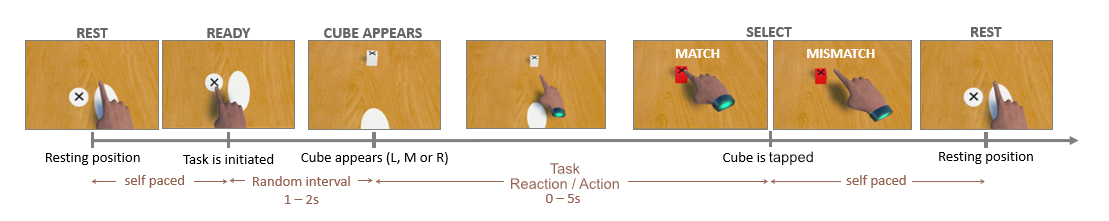
\includegraphics[width=\linewidth]{figures/Task_mismatch.jpg}
\vspace{-15pt}
\caption{Interaction flow depicting one trial in our 3D reach-to-tap task.}
\label{task_flow}
\end{figure*}

\subsection{Task}
Participants performed a 3D reach-to-tap task in VR designed with Unity Software (Unity Technologies, San Francisco, USA). The interaction flow of our task, depicted in Figure~\ref{task_flow}, was as follows: (1) participants moved their hands from the \textit{resting position} to the \textit{ready position}, to indicate they were ready to start the next trial; (2) participants waited for a new target to appear (the time of a new target spawning was randomized between 1-2 s); (3) then, the target (a cube) would appear in one of three possible positions (center, left, right), all equidistant from the participant's \textit{ready position}. \textcolor{n}{A black cross on the top of the cube indicated the location participants were instructed to tap};
(4) then, participants \textcolor{red}{\st{acquired}} \textcolor{n}{completed} the task by moving and tapping the target with their index finger. \textcolor{n}{Tapping success was, at least, indicated by a color change of the cube, see below for a detailed explanation of the feedback conditions.} (5) After a target was \textcolor{red}{\st{acquired}} \textcolor{n}{tapped}, participants moved back to the \textit{resting position}. Here, they could take a break before the next trial.

\textcolor{n}{To maximize EEG data quality, participants were instructed to remain in a calm upright seated position while carrying out the reaching movement. Further, they were instructed to be precise and keep a comfortable pace. However, no feedback was given on the accuracy and speed of their task completion.}

\subsection{Interface conditions}
Participants performed the task in two additive feedback conditions:

(1) \textbf{Visual-only (Visual)}: When participants tapped the cube, it changed its color from white to red (visual feedback.)\\
\indent(2) \textbf{Visual with vibro-tactile (Vibro)}: When participants tapped the cube in the Vibro condition, they received a 100 ms vibro-tactile stimulus with the color change (Visual + vibro-tactile feedback).
% \indent(3) \textbf{visuo-tactile plus force-feedback (EMS)}: in this condition, participants also received a 100 ms of EMS stimulation at the index finger extensor in addition to the visual and vibrotactile feedback (visual + tactile + force feedback)

\textcolor{n}{In this paper, our key focus was the calibration and source localization of a system detecting unrealistic VR interactions such as visual glitches or visuo-haptic synchronization errors. To maximize statistical power for the focus of our investigation we pooled trials from the two interface conditions. In order to build a stimulus-agnostic classification system detecting unrealistic system behavior, we chose to subject the pooled data to the cross-validation-- and localization method.}

\subsection{Introducing Visuo-Haptic Mismatches}
To allow us to compare the event-related EEG and movement signatures in a realistic vs. unrealistic interaction, we presented participants with two different classes of trials: \textbf{match trials (C)} (75\% of the trials) and \textbf{mismatch trials (M)} (25\%). This procedure elicits a prediction mismatch signal in 25\% of the trials similar to previous designs investigating the impact of target probabilities~\cite{Polich2007-cf}.  %on ERP modulations

In the \textbf{matching} trials, the feedback stimuli were presented upon tapping the object, exactly when participants expected them to occur based on the available visual information (finger touching the target in the virtual environment). In contrast, in the \textbf{mismatch} trials, the feedback stimuli were triggered prematurely, which was accomplished by enlarging the invisible radius of tap detection \textcolor{n}{(collision volume around the cube object)} by 350\%. While in the match trials, we used a collision detection volume of the exact size of the VR cube, in the mismatch trials, we used a larger sphere for collision detection. Our enlargement of the collision detecting volume was based on the study design by Singh et al.~\cite{Singh2018-qi}, in which they showed that VR users can detect a visual mismatch at around 200\% of offset from the target. In our pilot tests, we decided to extend the offset to 350\% to make the mismatch more obvious so as to provoke more pronounced prediction errors. 

We used a match-to-mismatch ratio of 75\%-25\% of the total trials by modeling our study after previous studies, which also ensured that participants were faced with a detectable unrealistic behavior of the virtual environment~\cite{Liao2011-po,Wiersema2007-jf,Donchin1988-gq}. For these unrealistic trials to occur, the participants must first be able create a stable model of how the VR world operates, thus the VR world cannot behave at a random 50\%-50\% match-mismatch ratio. 

Finally, these match vs. mismatch trials were presented in five \textcolor{n}{pseudo-}randomly generated sequences. \textcolor{red}{\st{, each with an equal distribution of matches and mismatches.}} \textcolor{n}{Following each mismatch trial, the next trial was always a match trial. To reduce the predictability of when the next mismatch trial would occur, the number of consecutive match trials was pseudo-randomized between 1 and 5.}

\subsection{Experimental design}
The experiment consisted of five phases: (1) a setup phase; (2) a calibration phase; (3) a short training phase; (4) the task itself, in all three possible interface conditions, each followed by a subset of items from the IPQ questionnaire (G1, REAL2, SP4 and INV1)~\cite{Schubert2003-sq} and the NASA-TLX~\cite{Hart1988-iw}. Lastly (5) participants were asked about their experience in the VR and which condition they enjoyed the most.

For training purposes, we asked participants to wear the HTC VIVE VR headset for a maximum of 24 practice trials. Overall, the EEG fitting, calibration, and practice trials took around 30 minutes \textcolor{red}{\st{(with two experimenters)}}. 

Next, we recorded a within-subjects design with 300 trials for each the Visual and Vibro feedback condition. The order of the Visual and Vibro conditions was randomized across participants. \textcolor{n}{We chose to present the two interface conditions in a blocked design. This was done to emphasize the influence of the additional haptic channel while attenuating higher order interactions, such as a prediction error about the upcoming interface condition.}

%%%%% LG writing resources:

% Next, we recorded a within-subjects design with 300 trials for each the Visual and Visuo-Tactile feedback condition, and 100 trials for the EMS condition. The order of the Visual and Visuo-Tactile conditions was randomized across participants with the EMS condition always being the last block. This was done to avoid potential overshadowing of the EMS stimulation (a very strong sensation) on the two other stimulation conditions.

% \subsection{Task and Procedure}
% Using an HTC Vive VR Headset with the Vive Deluxe Audio Strap and a Vive Tracker (HTC Corporation, Taoyuan, Taiwan) attached to the right hand, a 3D object selection task was presented on a virtual table placed on an infinite white plane. The virtual environment was created in the Unity3D engine (Version, company details). White cubes appeared at random either in the center, to the left, or to the right of the participant, equidistant from a starting position (see Figure ??). The time of a new cube spawning was randomized between 1-2 seconds after starting a trial. 

% %no subsections? This so hard to parse, make a task heading or so?
% Participants were tasked to select the cube with their index finger and, upon completion, move their hand back to a resting position indicated on the table. The task was completed in two blocks of 300 trials each, with one block providing visual-only feedback, i.e. the cube changing its color from white to red upon selecting, and one block providing visual-tactile feedback, in which the selection contact was indicated by the color change plus a small vibrotactile pulse. Placed under the index fingertip, a vibration motor (Model \textit{308-100} from \textit{Precision Microdrives}), generating 0.8g at 200Hz and measuring 8mm in diameter was driven at 70mA by a 2N7000 MOSFET connected to an Arduino output pin at 3V. An initial 24 trial training session was followed by the two experimental blocks (balanced across participants), each followed by two questionnaires, NASA-TLX and IPQ. For the main experimental manipulation of asynchrony, 25\% of the trials (totalling 75 asynchronous trials per feedback block of 300 trials) exhibited spatio-temporal asynchrony in line with established oddball paradigms. Object selection was triggered prematurely by bounding a spherical collider to the cube and enlarging it by 350\% in comparison to a collider bounded to the shape of the cube in the synchronous trials. Asynchronous trials were sorted in a pseudo-randomized sequence following synchronous trials, i.e. between one and five synchronous trials preceeded an asynchronous trial. Extended task and apparatus descriptions can be found elsewhere \cite{Gehrke2019}.
% % todo add movie, figure and references

\subsection{Dataset}

\subsubsection{Participants}
20 participants (12 female, mean age = 26.7 (sd = 3.6)) were recruited through an online tool provided by the Department of Psychology and Ergonomics and through local listings. Participants were right-handed, had normal or corrected to normal vision and had not experienced VR with vibro-tactile feedback at the fingertip. Participants were compensated with 10 Euros per hour or 1 study participation hour (course credit). Participants were informed of the nature of the experiment, recording and anonymization procedures and signed a consent form approved by the local ethics committee of the Department of Psychology and Ergonomics at the TU Berlin (Ethics approval: GR\_10\_20180603). Data of the first subject had to be removed from further analyses due to data recording error.

\subsubsection{Recordings: Motion Capture and EEG}
EEG was recorded using 64 active Ag/AgCl electrodes placed according to the extended international 10–20 system \cite{Chatrian1985-ys}. The electrode at position FP2 was detached from the cap and placed under the left eye to provide additional information about eye movements (EOG). Impedance was kept under 5k$\Omega$ where possible and the EEG was sampled at 500 Hz and amplified using BrainAmp DC amplifiers (Brainproducts GmbH, Gilching, Germany). Hand and head movements were sampled at 90 Hz when coming out of the HTC Vive processing cascade. EEG, motion capture and an experiment marker stream were recorded and synchronized using labstreaminglayer \footnote{https://github.com/sccn/labstreaminglayer}.

\subsubsection{Reproducing Results and Data Availability}
Data, experimental protocol, analyses code including scripts for a reproduction of the presented results and earlier publications are accessible from a comprehensive repository hosted at open science foundation (OSF)\footnote{https://osf.io/x7hnm/}. BIDS formatted data is hosted on openneuro \cite{ds003846:1.0.0}.

% Where applicable, EEG data was shifted by the \textasciitilde 50 ms age-of-sample of the recording setup to allow accurate comparisons of our EEG data with the literature\footnote{https://wiki.bpn.tu-berlin.de/wiki/doku.php?id=lab:lab_software:lsl:lsl-test}.
\subsection{Processing}

% \textcolor{red}{\st{\subsubsection{Predicting VR glitches using Behavioral Adaptation}}}
\subsubsection{Behavioral Adaptation Following VR Glitches}

Motion capture data was filtered with a 6Hz low-pass filter and re-sampled to match the EEG sample rate using MoBILAB routines for concurrent analyses~\cite{Ojeda2014-ev}. Subsequently the first derivative was computed and velocity was extracted. 

We computed `tap time', the time elapsed between the start of the reaching movement following object spawn and the end of that movement, using the hand velocity time series. The reach onset was detected on the hand velocity time series by moving backwards from the velocity peak of the reach movement and selecting the first sample where the velocity fell below 0.05 m/s. The end of the reach was determined as the first sign reversal of the movement change in z-direction, the primary reach direction, following the start of the reach. As such, tap time was detected on the continuous time series and not on the experimental event. This would have been problematic since the premature appearance of the mismatch feedback event would have artificially created an effect.

To assess behavioral adaptation, we modeled the \textit{rate of change} in `tap time' with a linear model. To this end, we computed the difference in `tap time' between subsequent trials and report this \textit{rate of change} as a response to the experimental manipulation~\cite{Dutilh2012-ps}. We reported tap time instead of reaction time since participants were not primed, nor did they receive any reward for fast and accurate trial completion. The model \textit{`change in tap time $\sim$ trial change'} was fitted using Matlab's `fitlm' function and assessed using `anova'. Trial change was entered as a categorical predictor reflecting whether the current trial change was match to mismatch, mismatch to match or match to match. Since the number of consecutive match trials was pseudo-randomized between 1 and 5 we decided to exclude trials where a mismatch trial occurred again after the first subsequent match trial. These trials corresponded to both the mismatch to match and match to mismatch trial change category. This resulted in the removal of 30 Trials per participant for the behavioral analysis.

%`Sequence' described the number of consecutive match trials preceding a mismatch trial. The current `sequence' value at each mismatch trial was applied to both the match to mismatch as well as the subsequent mismatch to match trial. 

% \textcolor{red}{\st{We modeled the occurrence of match/mismatch trials with a generalized linear (mixed effects) model employing the \textit{rate of change} in tap time as a predictor. The model \textit{`Feedback $\sim$ change in tap time + (1 | Participant ID)'} was fit using Matlab's `fitglme' function. To assess the model, we calculated a variance-ratio test using Matlab's `compare' function. In order to comply with the ERP classification scheme outlined below, we randomly sub-sampled trials from the match class to match the trial count in the mismatch class. The predictive accuracy of the model was assessed using a within-subject 5-fold cross-validation. In the within-subject case, the model is identical to a generalized linear model \textit{`Feedback $\sim$ change in tap time}. To assess the models effectiveness, a two-sample T-test was computed using participants average accuracy across folds and the simulated chance level under consideration of the classes sample size}}~\cite{Muller-Putz2007-oc}.

\subsubsection{Brain activity: EEG Preprocessing, Independent Component Analysis (ICA)}
EEG data preprocessing and ICA were performed in Matlab 2019b (MATLAB, The MathWorks Inc., Natick, MA, USA), using the EEGLAB toolbox~\cite{Delorme2004-sn} and custom `BeMoBIL Pipeline' scripts and functions. To detect bad channels for rejection, the `FindNoisyChannel' function was used, which is selecting bad channels by amplitude, the signal to noise ratio and correlation with other channels ~\cite{Bigdely-Shamlo2015-ds}. Rejected channels were then interpolated while ignoring the EOG channel, and finally re-referenced to average reference (data A). The data was then filtered with a 1 Hz high-pass filter (data B) and a first adaptive mixture independent component analysis, AMICA~\cite{Palmer2011-zs}, was used to identify eye related independent components (ICs) which were projected out of the sensor data. For this, the rank was reduced by one for the use of an average reference and further by the number of interpolated channels in the respective data set. To identify eye components, IClabel~\cite{Pion-Tonachini2019-fy} was used, whereas components exceeding a value of 0.7 for the 'eye' class were defined as eye components. Then, to detect segments of noisy data, an automated time domain cleaning (see~\cite{gramann2021human}) was performed on narrowly filtered data from 1 to 40 Hz. The data was therefore first split into 1 second long segments for which the mean absolute amplitude and standard deviation of all channels as well as the Mahalanobis distance of all channel mean amplitudes were calculated. All three methods results were then joined together in order to rank all segments. The 12\% highest ranking noisy segments were selected for rejection and an additional buffer of $\pm 0.49$ sec was added around each segment resulting in about 15\% rejected data for each subject. This data was rejected from data B and a second AMICA was calculated on this time domain cleaned data. A dipole fitting procedure was performed for each spatial filter using the 10-20 standard electrode locations and a boundary element head model (BEM) based on the MNI brain (Montreal Neurological Institute, MNI, Montreal, QC, Canada). The spatial filter information was then copied back to the preprocessed, interpolated and average referenced data set (see description of data A above).

To obtain indices of clean tap epochs, we leveraged EEGLAB's `pop\textunderscore autorej' function to remove epochs exhibiting large amplitude fluctuations. We used the functions default settings and entered epochs from -3 to 2 seconds surrounding the tap events. On average, 80.7 epochs were rejected (SD = 32.6) amounting to $\sim$13\% of the data.

Ultimately, all ICs with a probability smaller than .7 as indicated by the ICLabel `brain' class were projected out of the data. This resulted in the final dataset including only very likely brain sources and their projections to the channels. Across the study set, 271 independent components were retained forming a representative sample of about 14.3 (SD = 5.0) components per participant. All subsequent EEG analyses were based on these data.

\subsubsection{EEG Classifier, Classifier Scalp Projections and Localization of Components relevant to Classification}

In the current work, we present a processing pipeline with slight updates as compared to our earlier work~\cite{Gehrke2019-og}. To reproduce our previous findings, we report a permutation t-test of the ERP at electrode FCz. Activity at electrode FCz in the time window from 150 to 200 ms post mismatch event featured prominently in our earlier analysis and is frequently considered for MMN paradigms investigating ERPs at the scalp level, for modeling evidence see~\cite{Lieder2013-dl, Lieder2013-os}. For completeness, we report all electrodes that exhibited an amplitude difference at 200 ms post tap event. To this end, we computed a t-test of the amplitudes at 200ms post tap event. To correct for multiple comparisons, the false discovery rate (\textit{fdr}) was computed with alpha = 05~\cite{Benjamini1995-cw}. Channels whose p-value exceeded the \textit{fdr} were plotted, see figure~\ref{erp}.

For classification of single-trial ERPs, we followed the approach introduced by \cite{Zander2016-ed}. A regularized linear discriminant analysis classifier was trained per participant with all mismatch trials constituting class 1 and a random sample of an equal number of match trials labeled class 2. Using the open-source toolbox BCILAB ver. 1.4, the classifier was trained on windowed means as features. First, EEG data were re-sampled to 100 Hz and band-pass filtered from 0.1 to 15 Hz. Average amplitudes of all channels in eight sequential 50 ms time windows between 0 and 400 ms after the cube was tapped were extracted as the windowed means feature vectors. A mean baseline taken in the -50 to 0 ms window was subtracted in order to compensate for event classes, match and mismatch, occurring at different stages of the ongoing movement. For robust performance estimation, a 5 x 5 nested cross-validation was used to calculate the shrinkage regularization parameter and assess the classifiers performance.

Classification accuracy was statistically evaluated using a two-sample T-test with the mean classifier accuracy per participant across folds and simulated chance level given trial numbers in each class \cite{Muller-Putz2007-oc}.

In order to learn what regions of the brain the classifier specifically relied on, we first transformed the LDA filters at each time window to LDA patterns reflecting a mixture of scalp activations with regards to the discriminative source activity \cite{Haufe2014-do}. Subsequently, each independent component's relevance for classification was computed as the dot product of the LDA patterns per time window and the ICA unmixing matrix filter weights~\cite{Zander2016-ed}. The equivalent current dipole models of independent components were then weighted by their relevance and ultimately visualized via EEGLAB `dipoleDensity' plots \cite{Krol2018-cw}. The Harvard-Oxford atlas was consulted to extract cortical labels of regions of interest \cite{Makris2006-kp}.




%%%%% resources [do not review]
% old:
% Using Matlab's `fitlme' function, the model \textit{`action time \textasciitilde  Feedback * Haptics + (1 | Participant Id)'} was fit to assess the alteration of 'action time through the experimental manipulation. Similarly, the model \textit{`change in action time \textasciitilde  Feedback * Haptics + (1 | Participant Id)'} was fit to assess post-error slowing. `Feedback' differentiated match from mismatch trials and `Haptics' vibrotactile from those missing the added immersive channel. Next, the occurrence of match/mismatch trials was modeled with a generalized linear mixed effects model employing the \textit{rate of change} in action time. The predictive accuracy of the model was assessed using 10-fold cross-validation \textit{across} participants. To assess the models effectiveness, a two-sample T-test was computed using each fold's accuracy and the simulated chance level considering the classes sample size in each fold~\cite{Muller-Putz2007-oc}.

% \subsubsection{Modeling Event-related Spectral Perturbations in "Midcingulate" Independent Components}
% % Linear modeling of Clusterwise Event-related Spectral Perturbation
% % specify the model and briefly state to what end it was designed, which questioned it was supposed to answer 

% \subsubsection{Single-Trial Multiple Regression, Group-level Statistics and Multiple Comparison Correction}
% In order to describe task execution relevant components of the event-related spectral perturbations of the entire epoch, we conducted a t-test of the grand average cluster ERSP, baseline corrected using grand average divisive baseline. Employing a permutation t-test using the function \textit{statcond} with 1000 permutations we controlled for multiple comparisons. Due to the small sample size (N = 17) we chose the permutation-t approach over a cluster statistic with constrained resampling \cite{Pernet2015}. This procedure was also used to assess inference of betas obtained from mass-univariate single-trial regressions as described below. With respect to the grand-average, slight shifts preceding the event of interest due to randomized pre-trial intervals were ignored and averaged across. This smearing in time was accepted since time-frequency resolution similarly reduces temporal accuracy. Since single-trial analysis only focused on the interval succeeding the event of interest, that is the feedback associated with touching the cube or, in case of mismatch trials, the premature feedback, randomized pre-trial intervals did not impact these analyses.
% % todo % citation statcond (fieldtrip and eeglab)
% %In order to correct for multiple comparison we transformed the resulting map of t-scores to a map of tfce-scores and thresholded the tfce-map at the 95th percentile of the max-tfce distribution of 600 bootstrapped t-tests using as implemented in LIMO EEG. Due to the low number of 17 participants in each analysed cluster, we constrained bootstraps to contain at least 14 unique participants to overcome conservative multiple comparison correction \cite{Pernet2015}.

% % better split grand-average and single-trial analyses
% \subsubsection{Single-trial regression to disentangle spatio-temporal binding prediction errors}
% To obtain first-level, per participant, summaries of event-related spectral perturbations, mass-univariate multiple regression was computed across all mismatch trials. Therefore, a linear model was estimated at each time-frequency pixel of participants independent component(s) present in the ROI cluster. The linear model was defined as \textit{tf\textunderscore pixels = intercept + hand\textunderscore velocity * haptic\textunderscore feedback + RT + Baseline}. Instantaneous hand velocity was extracted at the moment of object selection. Haptic feedback differentiated trials including vibrotactile from those missing the added immersive channel. In order to estimate the interaction term between hand velocity and haptics, both predictors were normalized prior to model fitting. Reaction time was operationalized as the time elapsed from the object spawning on the table to the object being selected. To further infer whether components of the event-related response could be explained by baseline activity, average power per frequency bin in the -200 to 0 ms window preceding cube \textit{spawns} was entered as a predictor as well.
% %optional if results are promising -> \subsection{correlation post-error slowing and theta}

% \subsubsection{Velocity perturbations following spatio-temporal binding prediction errors}
% To investigate whether ongoing motor behavior following spatio-temporal binding manipulations changed as a function of time or in response to haptic feedback a mass-univariate multiple regression was computed across all mismatch trials. The linear model \textit{velocity = intercept + trial\textunderscore number * haptic\textunderscore feedback} was fit at all time points addressing whether (a) trials were comparable across time and (b) whether rendering the surface by means of tactile feedback impacted movement execution potentially hinting at perceived object rigidity. At the group-level, a robust one-sample t-test was computed for betas of trial number and haptic feedback. To assess whether initiation and motor execution slowed down following spatio-temporal binding perturbations per participant betas were obtained by fitting the linear model \textit{velocity = intercept + following\textunderscore asynchrony * following\textunderscore haptics} at all time points across the epoch followed by group-level inference as described above.

% no overlapping ICs in clustering twice, one parietal, one visual association
% old solution
% (weight=6), grand-average ERSPs (weight=3), mean log spectra (weight=1), and scalp topography (weight=1),
 %The weighted IC measures were reduced to a 10-dimensional feature vector for clustering via PCA. 
 
 % maybe add movie for supplement material
% todo cite dipoledensity
%\footnote{Available at https://sccn.ucsd.edu/wiki/EEGLAB_ Extensions_and_plug-ins}
%and $[20, -65, 30]$ 
% make clear that class size was subsampled

% On average 83.7 (sd = 37.6) trials were removed. For each remaining single trial we considered event-related potentials for channels and independent components (ERP), event-related velocities, i.e. the magnitude of velocities in x, y and z direction (ERV) as well as event-related time-frequency decompositions (event-related spectral perturbation, ERSP). Time-frequency decomposition were computed via the \textit{newtimef} function in EEGLAB for 3 to 80 Hz in logarithmic scale, using a wavelet transformation with 3 cycles for the lowest frequency and a linear increase with frequency of 0.5 cycles. Subsequently, phase was discarded and raw power values were kept for further analysis. Where applicable, grand average ERSPs are computed by first averaging both trial data and baselines across trials in power then dividing trial data by baseline and transforming the outcome to logarithmic scaling ($dB = 10*log_{10}(power)$). ERPs are plotted after bandpass filtering with a low and high cutoff at 0.1 and 15 Hz respectively.


% % results

\section{Results}

Participants reached towards the target object after it appeared on the table. In the match trials without visuo-tactile VR glitches, participants took on average 1.04s (SD = .19) to complete the reach-to-tap. \textcolor{red}{\st{In the mismatch trials with visuo-tactile VR glitches, the target feedback was presented prematurely and triggered on average after .73s (SD = .12) following object spawn, see figure 1b.}}

\textcolor{n}{We created visuo-tactile VR glitches by increasing the (bounding) object volume of the target. Hence, the collision detection registered prematurely. In these mismatch trials, participants took on average .73s (SD = .12) to complete the reach-to-tap, see figure~\ref{setup_and_behavior}b.} Hence, increasing the (bounding) object volume for collision detection led to a spatio-temporal mismatch of approximately 300 ms as compared to the congruent, match, condition. The velocity profile in both conditions exhibited a narrow peak during outward reaching with a peak magnitude of ~.6 m/s and a broader and lower peak when the hand was retracted back to its origin, see figure \ref{setup_and_behavior}b bottom.

\begin{figure}[!h]
  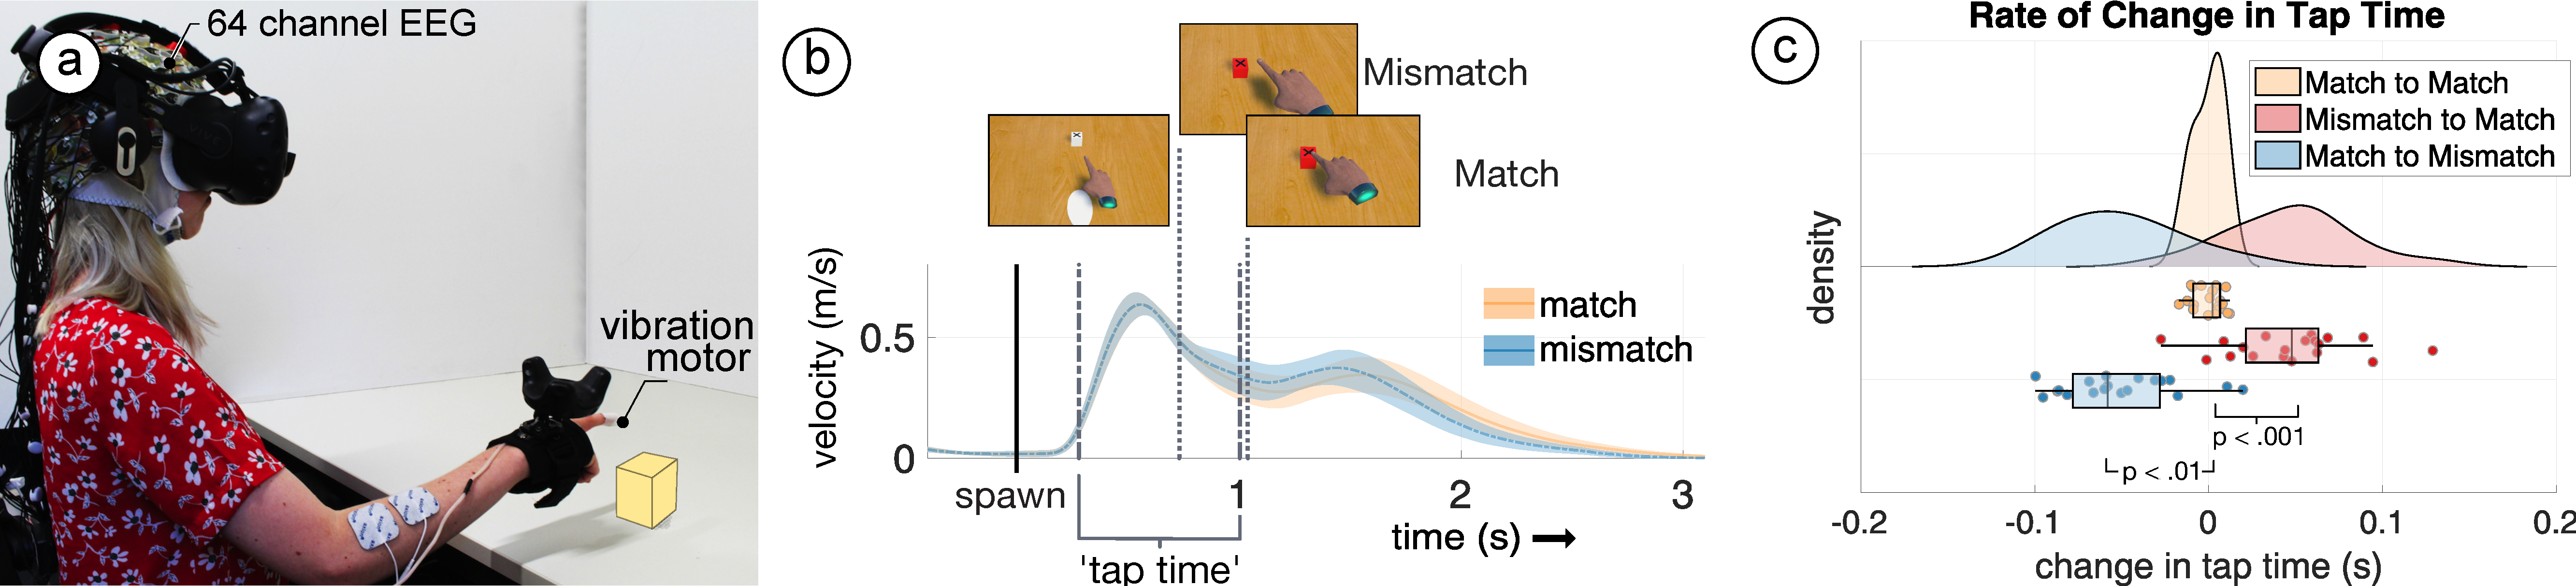
\includegraphics[width=\textwidth]{figures/task_behavior_new.pdf}
  \caption{Task Structure and hand velocity profile. \textbf{a} Participants were instructed to reach to an appearing cube on a desk in front of them and tap it. They were equipped with a VR headset, a 64 channel EEG cap, electrode spacers and rigid body tracker on the hand. The vibration motor was placed under the fingertip of the index finger. \textbf{b} Top: Inside VR view of experimental scene. Bottom: Grand-average velocity with 95\% confidence interval of both, match and mismatch conditions with event markers for object `spawn', tap time start and end as well as moments of object tap in match and mismatch conditions. \textbf{c} Distribution of \textit{rate of change} in tap time \textcolor{n}{for the three trial change categories `match to match', `mismatch to match' and `match to mismatch'.}\textcolor{red}{\st{between two subsequent match trials and following a VR glitch.}} A dot represents the average per participant per condition.}
  \label{setup_and_behavior}
\end{figure}

\subsection{Prolonged Tap Time Following VR Glitches}

% add a sentence that we now look at the corrected behavior computed on the velocity time series
\textcolor{n}{}

`Tap time', the hand movement period from movement start to reaching the object, lasted on average .74s (SD = .15) in match- and .69s (SD = .15) in mismatch trials. 

We calculated the \textit{rate of change} in `tap time' as a metric of post-error slowing \textcolor{n}{and observed that trial change categories impacted `tap time' ($F_{(2)} = 53.7, p < .001, R^2 = .66$). Following match trials, `tap time' in the subsequent trial did not change, i.e. 0 ms (SD = 20 ms). However, following mismatch trials, `tap time' was increased in the subsequent trial on average by} \textcolor{red}{\st{.05s (SD = .04)}}\textcolor{n}{47 ms (SD = 37 ms, $t_{18} = 5, p < .001$)}. \textcolor{n}{For completeness, `tap time' decreased from match to mismatch trials on average by 50 ms (SD = 33 ms, $t_{18} = -5.4, p < .001$).}

\textcolor{red}{\st{this modulation was about 48 times more likely to occur under the model considering mismatch modulation than the null model (equivalent ${\chi}^2_{(1)} = 48.1, p<.001$), see figure}~\ref{setup_and_behavior}c.}

% Using the trial-to-trial adaptation in tap time, trial classes (match/mismatch) were classified with an average within-subject classification accuracy across folds of 55.4\% (SD = 4.8), remaining below the significance threshold of the simulated chance level at 63.4\% (SD = 0.6).

% \footnote{For completeness, we also report a classification scheme using behavioral data of all trials, maintaining unequal trial numbers per match and mismatch condition. We found that using data from all trials and maintaining unequal class sizes increased the classification to $\sim$67\% accuracy. See the supplementary material for more detail.}









%%%% writing resources
% Frage: wenn vel profiles mit movement onset aligned dann sollten evtl. kurven gleich sein, es sei denn es gibt einen "kontinuierlichen" rekalibrationseffekt ist in den syncs. mit drin
% im idealfall ist der rekalibrationseffekt 1/4 der 300ms
% Optimierungsprozess um den RMSE bei rekalibration zu optimieren
% mallot VR noise adaptation
% The addition of a haptic sensation while taping the virtual objects (by means of vibrotactile stimulation) led participants to generally move their hand slower during the whole trial, see \ref{setup_and_behavior} C middle row. Participants started their outward movement earlier and their outward peak magnitude was lower when approaching the target (for example at 50 ms preceding object selection, $t_{18} = -2.14, P = .03$). Following trials with spatio-temporal asynchrony, movement behavior was altered in the next trial. An earlier movement onset with a broader peak and immediate retraction following object select was observed (for example at 100 following object selection, $t_{18} = -17.24, P = 0$). Taken together, the task introduced spatio-temporal asynchrony, with rendered vibrotactile feedback as well as the asynchrony impacting future reaching movement characteristics.

\begin{figure}[h]
  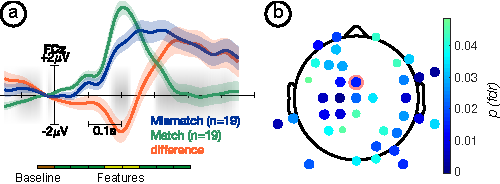
\includegraphics[width=.7\textwidth]{figures/erp_FCZ_diff_delay_with_scalp_map.pdf}
  \caption{\textbf{a:} Grand-average ERP (n = 19) of projected source mixtures at electrode FCz with significant class differences marked in grey. Bottom: Time windows used to compute features for classification (all greens). Windows in light green indicate time windows of interest for classifier source localization. \textbf{b:} Electrodes with a significant amplitude difference (\textit{fdr} corrected) between match and mismatch trials at 200 ms post tap event. Electrode locations are color scaled by their respective p-value, colder colors correspond to a lower p-value. Scalp location of electrode FCz (see subplot \textbf{a}) is highlighted with a red background.}
  \label{erp}
\end{figure}

\subsection{$\sim$77 \% Classification Accuracy Detecting VR Glitches using ERPs}

We found significant differences between match and mismatch trials in the grand-average event-related potential (ERP) at several scalp locations, see figure \ref{erp} showing the ERP at electrode `FCz' for an example. Hence, we reproduced our previous findings in \cite{Gehrke2019-og} with an altered processing pipeline. At electrode `FCz', amplitude differences at 200 ms indicated a significant difference between mismatch, i.e. the VR glitch condition and the matching trials ($t_{18} = -5.34, p < .001$). Differences were observed most strongly in the 150-280 ms time window, at 250 ms and in later windows starting at 350 ms, see figure \ref{erp}.

To assess the potential for single-trial online applications, a discriminative classification system was cross-validated. The system, using windowed mean ERP features, succeeded in detecting VR glitches. Mismatch and match trials were correctly labeled to the corresponding class with an average accuracy of $\sim$77 percent ($SD = 9.12$). The classification accuracy exceeded chance level at $\sim$ 56 percent, $t_{(18)} = 42.1, p < .001$. 

\subsubsection{Classification Driven by Midline Cingulate and Occipital EEG Sources}

To draw conclusions about the cortical origin of the discriminatory signal we investigated which EEG sources contributed maximally to the classification. With regards to the system's applicability as robust neural interface technology, this source reconstruction served two purposes: (1) Asserting that the classifier did not rely \textit{primarily} on artifact EEG sources, and (2) to gain additional information about the contributing brain regions to allow interpretations about cognitive processing.

In the fourth time window of the eight windowed mean features (150 - 200 ms, see the first light green shaded window at the bottom of figure \ref{erp} and in figure \ref{lda_loc}a top) classifications were driven primarily by activity originating in right lateral parieto-occipital cortical sources (BA19; MNI: x = 30, y = -70, z = 30), see figure \ref{lda_loc}a bottom. In the following time-window (200 - 250 ms, see the second light green shaded window at the bottom of figure \ref{erp} and in figure \ref{lda_loc}b top) the classification signal draw from distributed source activity in occipital areas as well as from sources located in anterior midline cingulate gyrus (near BA23; MNI: x = 0, y = -10, z = 30), see figure \ref{lda_loc}b bottom. Some ocular sources were not classified as such by our automated processing pipeline and carried information relevant to classification in this time window of interest.

\begin{figure}[!h]
  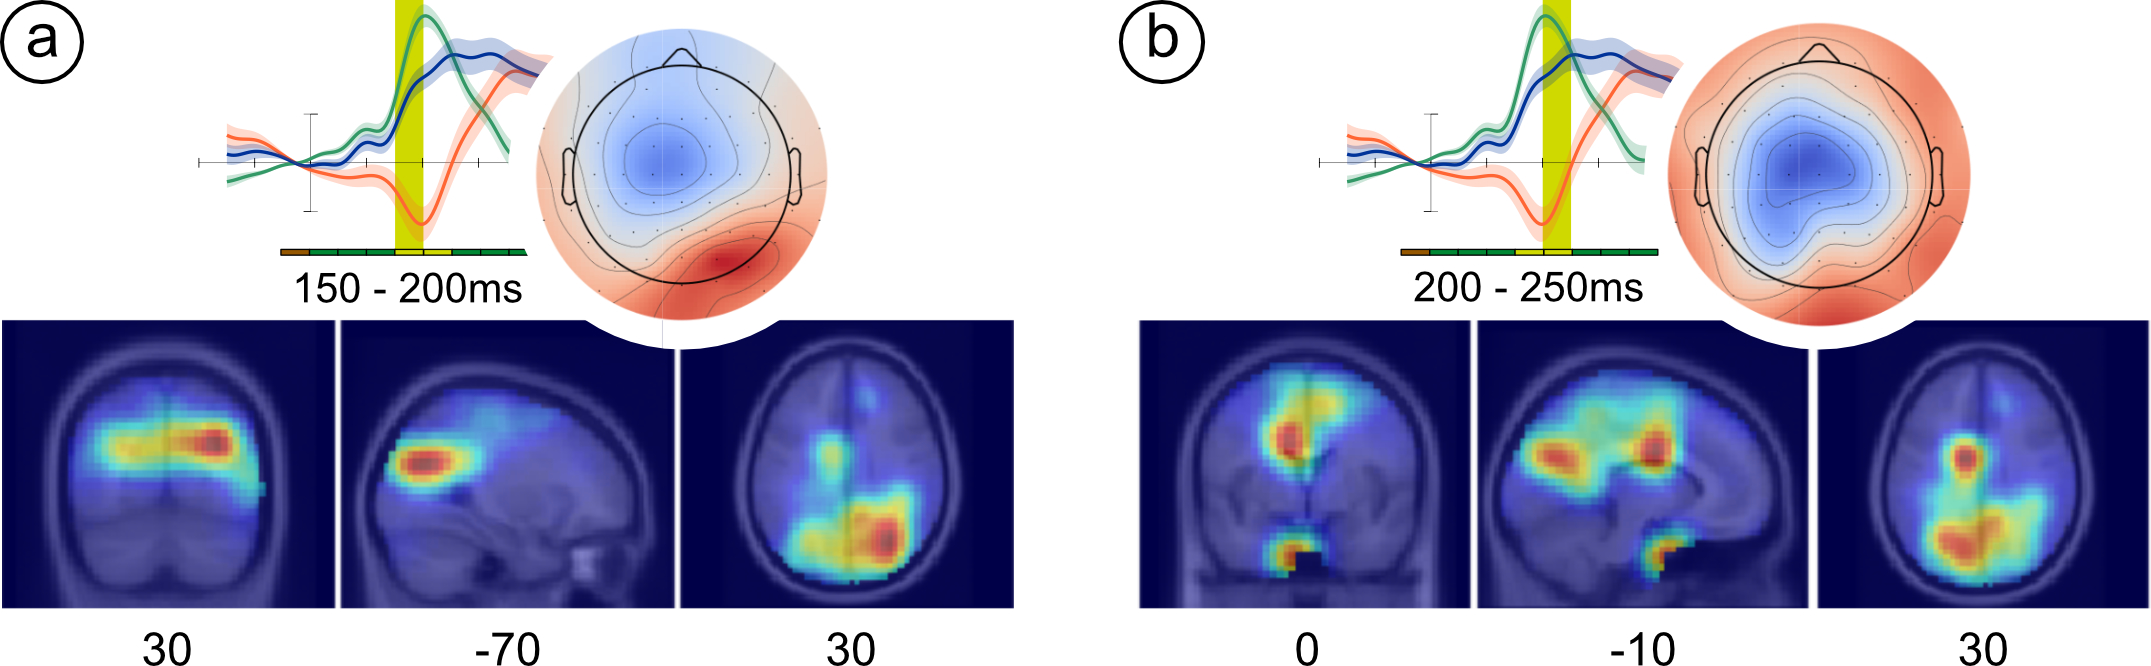
\includegraphics[width=\textwidth]{figures/fig_localization.jpg}
  \caption{An LDA classifier was trained on eight windowed means of 50 ms size from 0 to 400 ms following the cube tap, see figure \ref{erp} bottom. Two classes of synchronous and asynchronous trials were labeled for training and cross-validation. \textbf{a, b} Scalp maps of difference-between-classes activity for the 4th (150-200) and 5th (200-250ms) time windows and the equivalent source localization (MNI coordinates of the location of maximum activity).}
  \label{lda_loc}
\end{figure}

% discussion
% aim for 1500 words: 1473 -> nice, don't add, improve!
\section{Discussion}

%%% Statement/Summary of principal findings
With this study, we contributed a new approach to automatically detect conflicts in visuo-tactile sensory integration in VR based on a classifier using ERPs. 

Our work aimed at elucidating whether ERP-based classification can help address the challenge of \textit{continuous} labeling of a user's immersion. This work contributes towards the overarching goal to develop a continuous method to validate the effectiveness of haptic devices that foster presence experience.

We achieved a $\sim$77 \% classification accuracy detecting visuo-tactile glitches in a reach-to-tap task in VR. The midline cingulate cortex as well as a distributed network of parieto-occipital EEG sources enabled the classification success.

We believe our experimental setup, and/or data, can be used to calibrate a classifier that labels unrealistic VR interactions in near real-time. Consider the example of grabbing a hammer in VR with a game controller. When the available sensory channels are misaligned, for example the hammer `snaps' to the virtual hand before the controller's vibration simulates physical contact, the interaction is labeled `unrealistic' by the ERP-based classifier. When interacting with objects in VR, ERP-based classification is a promising endeavour due to the abundance of events.

% \textcolor{red}{\st{We discuss two noteworthy points: (1) the missing contribution of post-error movement adaptation to the classification and (2) challenges for BCIs relying on embodied predictive coding in natural interaction.}}
% \textcolor{red}{\st{We discuss two noteworthy points \textcolor{n}{about our findings}: (1) the missing contribution of post-error movement adaptation to the classification and (2) challenges for \textcolor{n}{ERP-based classification for} BCIs relying on embodied predictive coding in natural interaction.}}

%%% filling the gap detail #1
% \subsection{Using Post-error Adaptation to Detect Visuo-Tactile Mismatches during Interaction with Virtual Worlds}
\subsection{Post-error Adaptation Following Visuo-Tactile Mismatches during Interaction with Virtual Worlds}

% \textcolor{red}{\st{We explored whether a movement metric, post-error adaptation, can supplement the classification and motivate a multimodal approach}}.
We hypothesized a trial-to-trial adaptation in movement behavior as an implicit behavioral reflection of the effectiveness of our `VR glitch' experimental manipulation.~\cite{Dutilh2012-ps} have shown that correlations of brain signals with global averages of post-error slowing metrics may be moderated by confounding \textit{cognitive} processes, e.g. fluctuating concentration levels. Therefore, we looked at the rate of change in `tap time'. Between two subsequent match trials there was no change in `tap time'. However, `tap time' increased in the trial following a mismatch trial. Similarly, we observed a decrease in `tap time' in the mismatch trials following match trials. While the effect is comparable in absolute value to the increase in the `match to mismatch' trial change condition, we note that it is challenging to separate the processes underlying these changes in behavior. While one might happen more immediately due to the glitch manipulation, the other one may happen as a delayed consequence of it.

In general, these findings confirmed our manipulation, since the visuo-tactile VR glitch impacted behavior. Consequently, this ruled out the possibility of an automatic behavior in which participants were unaware of the manipulation. Since the task featured 600 trials, this was not unlikely. 

We believe our findings further evidence the literature on post-error adaptation, with participants taking a slightly more cautious approach following VR glitches~\cite{Rabbitt1977-yg}. This speed decline has frequently been observed to facilitate increasing accuracy on subsequent trials~\cite{Ridderinkhof2004-rz}. Here, cognitive control processes inhibit motor execution, presumably by closely monitoring, and raising, cortical activity thresholds~\cite{Botvinick2001-bs}.

In summary, we believe our data captures `prediction errors', violations of goal-directed behavior under consideration of the predicted action outcome. Further, we hypothesize cognitive control mechanisms to monitor and adjust subsequent motor output with one objective being an increase in behavioral accuracy. Only observing minor differences in absolute values between `mismatch to match' and `match to mismatch' may be due to the missing framing of our task: (1) not giving participants an incentive to optimize the speed-accuracy trade-off and (2) not providing any feedback on their task performance. Not collecting an accuracy metric is a shortcoming that should be improved in subsequent works, for example as in~\cite{Purcell2016-li}.

% \textcolor{red}{\st{However, due to the small effect size, our `tap time' metric did not enable a successful classification as compared to the EEG features. The low behavioral classification rate might be a consequence of the missing framing of our task, not priming participants on a speed-accuracy trade-off. Not collecting an accuracy metric is a shortcoming that should be improved in subsequent works, for example as in}~\cite{Purcell2016-li}.\st{ However, we note that increasing the amount of data subjected to the behavioral classification approach increased the accuracy of the classifier substantially (see supplementary material). In order to obtain robust cross-validated classification accuracy estimates, we chose to subject balanced classes to the cross-validation scheme and hence maintain a 50\% theoretical chance level.}}

%%% filling the gap detail #2
\subsection{Towards BCI based on Embodied Predictive Coding during Interaction with Virtual Worlds}

In order to describe a robust ERP feature representing prediction errors, we localized their EEG source origin and found two loci: (1) the midline cingulate cortex and (2) a distributed network in parieto-occipital areas. 

The role of midfrontal EEG source activity has frequently been linked to cognitive control processes~\cite{Ridderinkhof2004-rz, Cavanagh2014-mm, Cooper2019-im}. Crucially, these studies employed a stationary setup, limiting participants' interaction with the task environment. However, environmental affordances surpass the visual domain. Particularly in humans, a proclivity to use both hands to act on the environment has emerged and is greatly trusted upon, for example when finding your way in the dark~\cite{Gehrke2018-jm, Gehrke2021-ml, Miyakoshi2021-ni}. In fact, many tasks can be completed without concurrently consulting the visual domain, such as typewriting or even reaching for a cup; these typically rely heavily on the tactile and proprioceptive sense and as such are denoted as eyes-free interactions.

In our voluntary, albeit instructed, tapping task, we observed a frontal prediction error negativity, `PEN', (at electrode FCz) to exhibit a familiar time course as compared to stationary setups reporting MMN, see difference wave in figure \ref{erp}. In line with the MMN literature, we observed a stronger early negative deflection in mismatch trials as compared to the match trials, see figure \ref{erp}.~\cite{Zander2016-ed} report a single `PEN' source origin in anterior cingulate cortex, however in our study, besides midline cingulate sources, sources in parieto-occiptal areas contributed to the successful classification. Previously,~\cite{Savoie2018-ad} observed an effect of prediction errors about the visual consequences of the current motor action in a reaching task in parietal electrodes contralateral to the reaching hand. The authors conclude a role of the dorsal processing stream, processing the `where' in visuomotor `PEs'. Interestingly, first evidence now indicates that cortical cross-talk between the motor area corresponding to the active, for example reaching, hand and parietal regions may in fact reflect the strength of the body illusion in VR, the illusion that an avatar's hand is in fact mine~\cite{Casula2022-tq}. Considering the classifier weighting in our task in the time periods between 150 to 200 ms as well as 200 - 250 ms, we take note of a parieto-occipital reliance for match/mismatch separation in the earlier time window which was followed by a more pronounced weighting on frontal midline sources in a following time window.

Hence, we observed our classifier to first rely on parieto-occipital sources and subsequently on frontal midline sources in the typical time range of the MMN. This may indicate the role of embodied affordances in our immersive reaching task. Attention modulating cognitive control during `PEs' may be represented in the MMN. In stationary setups or `motor-passive' paradigms, such as in~\cite{Zander2016-ed}, no countermeasure to correct the `PE' exists. This may explain a heavy role of midline cingulate activity in classification with no other sources contributing. However, even for a simple task like reaching for an object, several sensory signals (e.g., visual, tactile and proprioceptive feedback) are continuously gathered and analyzed to efficiently interact with/in a dynamically changing environment. To compensate for the sensory noise within the nervous system and for the uncertainties in the dynamic environment different movement-related sensory cues have to be integrated. To gain an overall representation of the body position, movement and acceleration, the most reliable sensory information must be enhanced while the most noisy ones must be diminished~\cite{Fetsch2011-bp}, i.e. multisensory integration. With increasing immersion, processing gets more accurate and therefore might trigger a hierarchical cascade of `PE' processing~\cite{Singh2021-qc}. Here, multisensory integration in parieto-occipital regions precedes action outcome evaluation and cognitive control supported by midline cingulate cortex structures. However, the fact that our classifier relied on parieto-occipital source activity is direct evidence for `PE' processing. One possible explanation is that sensory `PEs' may already be resolved at early stages in the processing cascade instead of an inefficient signal forwarding to frontal brain areas.

%%% Limitations in filling the gap
\subsection{Limitations \& Open Challenges}

% \textcolor{red}{\st{Our classification results rely on the presence of a binary class label, `match' - `mismatch'. For online application where no such labels exist, this poses a problem. However, the presented paradigm may serve as a \textit{calibration}, with subsequent online application using a moving window providing a class probabilities. When a threshold is exceeded, the system trained on labeled glitches provides information on the current user experience of visuo-tactile congruency. It is interesting to follow up our investigation with regards to the level of haptic immersion. In}~\cite{Gehrke2019-og}\st{ we have shown a dependence of the level of haptic immersion on the `PE' early negative component. This hints at a potentially better classification accuracy with increasing immersion and is an objective for future research.}}

To allow for a full reproduction of our results, we provide the BIDS formatted data as well as all processing code alongside this publication. We chose automated over manual processing. However, problems remain in automated labeling of EEG sources. As evident in figure~\ref{lda_loc} sources localized to the eyes did contribute to the classification. More stringent vetting of EEG sources could make the results to rely exclusively on brain sources. However, using the eye activity features for classification is useful as long as it is reliable. This is especially relevant when using low-density EEG systems, such as consumer market products and it would be interesting to dissociate the different sources' contribution to the classification.

One way to validate `PEN' as a correlate of sense of presence would be a correlation with established presence questionnaires~\cite{Witmer1998-ew,Schubert2003-sq}. We believe that due to the highly repetitive experimental design and very subtle experimental manipulation, frequently asking questions would not yield valid results in the sense that frequently breaking the ongoing presence experience would bias the very construct we aimed at measuring. Recently~\cite{Grassini2021-tc} reported a correlation of late ERP components in central electrodes with the subjective presence experience. The authors used an auditory irrelevant probe paradigm and showed that ERP fluctuations to auditory distractor probes coincided with presence ratings. This approach relies on probing the user's overall attentional state. Instead, our proposed approach directly probes the user's internal model of their environment providing a precise task-relevant marker for neuroadaptive interfaces \cite{Krol2020-lj}.

Due to the high-level of immersion in VR, classifying event-related activity such as that occurring during object interaction, may be improved by an unfolding of overlapping activity. For example, when picking up a virtual hammer in VR, several `events' may co-occur. A visual event in the background may coincide with the haptic event of the controller when making contact with the hammer. The exact timing and rich descriptions of all such co-occurring events readily exist in VR simulations making near real-time overlap correction feasible. Novel approaches to `unfold' such EEG data exist~\cite{Ehinger2019-in}. We believe real-time ERP-based user experience classification in VR will benefit significantly from such overlap correction, amplifying the signal while attenuating the noise.

%%% 'Contributions beyond'
\subsection{Conclusions \& Outlook: Towards a Robust Metric of Presence Experience in Virtual Worlds}

Midline cingulate EEG sources contributed to prediction error ERPs, `PENs', and may serve as a robust source to detect violations of user's predictions about the interaction with virtual worlds~\cite{Gehrke2019-og, Si-mohammed2020-ru, Zander2016-ed}. This source origin can be specifically and repeatedly probed for real-time BCI purposes, informing the technical system about the user's mental representation generating the predictions~\cite{Krol2020-lj, Zander2016-ed}. If follow up studies replicate and extend on our classification success several benefits emerge: (1) the ERP-based measure to continuously evaluate haptic immersion gains significant robustness and reliability. (2) This will in turn motivate further research on the PE paradigm moving towards implicit measures of the user's subjective experience. (3) We believe this paves the way for fast and reliable real-time adaptation as the EEG feature search space is significantly reduced. However, our results also show a network of distributed parieto-occipital EEG sources contributing to the classification success. This indicates the challenges remaining in scenarios with a higher level of physical immersion. 

With this work, we hope to contribute to the design of a new method based on neural interface technology to assess the effectiveness of haptic devices that foster the emergence of presence experience.

% \textcolor{n}{specifically those to assess the effectiveness of haptic devices fostering the emergence of presence experience.}



%%% writing resources
% However, the predictive brain still receives noticeably less realistic sensory cues from the interaction with/in VEs when compared to the sensory richness of the physical interaction. Therefore, the multisensory integration processes needs to fill in more of the missing (or contradicting) sensory information by interpolating and augmenting the computer-simulated sensory information~\cite{Fetsch2011-bp}. Overall, integrating additional sensory modalities to the VE leads to an enhanced intersensory experience, so that the mental representation of the virtual world is more reliable and the level of presence is enhanced~\cite{Dinh1999-qe, Bohil2011-gu}.

\ack
This research was supported by a grant from the German Federal Ministry of Education and Research (01GQ1511) to KG

% supplementary material
% \section{Supplementary Material}

\subsection{Prolonged `Tap time' Following VR Glitches: Leveraging all trials for classification}

Subjecting all trials to the classification scheme, here we report results using the same analysis as in the behavioral part of the results section. Since we leveraged a 75\% to 25\% match to mismatch ratio this increased the amount of data significantly. `Tap time', the hand movement period from movement start to reaching the object, lasted on average .75s (SD = .15) in match- and .69s (SD = .15) in mismatch trials. 

We calculated the \textit{rate of change} in `tap time' as a metric of post-error slowing. Following match trials, `tap time' in the subsequent trial did not change, i.e. 0s (SD = .01). However, following mismatch trials, `tap time' was increased in the subsequent trial on average by .05s (SD = .04); this modulation was about 67 times more likely to occur under the model considering mismatch modulation than the null model (equivalent ${\chi}^2_{(1)} = 67.5, p<.001$), see figure \ref{setup_and_behavior}c.

\begin{figure}[!h]
  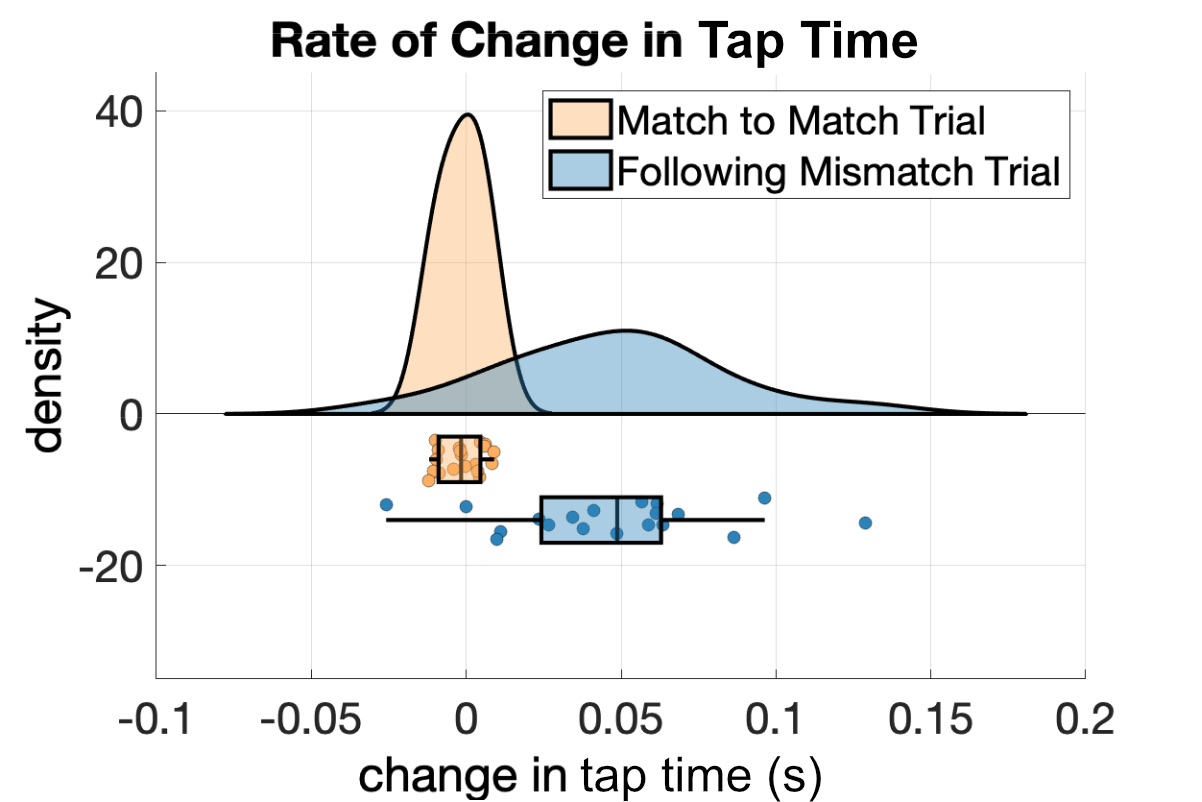
\includegraphics[width=.5\textwidth]{figures/rate_of_change_action_time_all_trials_.jpg}
  \caption{Distribution of \textit{rate of change} in `tap time' between two subsequent match trials and following a VR glitch. A dot represents the average per participant per condition. Here, all trial information is considered, maintaining unequal class sizes for match and mismatch conditions.}
  \label{behavior_supplements}
\end{figure}

Using the trial-to-trial adaptation in `tap time', trial classes (match/mismatch) were classified with an average within-subject classification accuracy across folds of $\sim$67\% (SD = 2.2), exceeding the significance threshold of the simulated chance level at $\sim$61\% (SD = 0.01, $t_{(18)} = 10.2, p < .001$.

% Submissions are not required to reflect the precise reference formatting of the journal (use of italics, bold etc.), however it is important that all key elements of each reference are included.
\section*{References}
\bibliographystyle{iopart-num}
\bibliography{references}

% \section{Introduction: file preparation and submission}


% The \verb"iopart" \LaTeXe\ article class file is provided to help authors prepare articles for submission to IOP Publishing journals.
%   This document gives advice on preparing your submission, and specific instructions on how to use \verb"iopart.cls" to follow this advice.  You
%   do not have to use \verb"iopart.cls"; articles prepared using any other common class and style files can also be submitted.
%     It is not necessary to mimic the appearance of a published article.

% The advice
% on \LaTeX\ file preparation in this document applies to
% the journals listed in table~\ref{jlab1}.  If your journal is not listed please go to the journal website via \verb"http://iopscience.iop.org/journals" for specific
% submission instructions.

% \begin{table}
% \caption{\label{jlab1}Journals to which this document applies, and macros for the abbreviated journal names in {\tt iopart.cls}. Macros for other journal titles are listed in appendix\,A.}
% \footnotesize
% \begin{tabular}{@{}llll}
% \br
% Short form of journal title&Macro name&Short form of journal title&Macro name\\
% \mr
% 2D Mater.&\verb"\TDM"&Mater. Res. Express&\verb"\MRE"\\
% Biofabrication&\verb"\BF"&Meas. Sci. Technol.$^c$&\verb"\MST"\\
% Bioinspir. Biomim.&\verb"\BB"&Methods Appl. Fluoresc.&\verb"\MAF"\\
% Biomed. Mater.&\verb"\BMM"&Modelling Simul. Mater. Sci. Eng.&\verb"\MSMSE"\\
% Class. Quantum Grav.&\verb"\CQG"&Nucl. Fusion&\verb"\NF"\\
% Comput. Sci. Disc.&\verb"\CSD"&New J. Phys.&\verb"\NJP"\\
% Environ. Res. Lett.&\verb"\ERL"&Nonlinearity$^{a,b}$&\verb"\NL"\\
% Eur. J. Phys.&\verb"\EJP"&Nanotechnology&\verb"\NT"\\
% Inverse Problems&\verb"\IP"&Phys. Biol.$^c$&\verb"\PB"\\
% J. Breath Res.&\verb"\JBR"&Phys. Educ.$^a$&\verb"\PED"\\
% J. Geophys. Eng.$^d$&\verb"\JGE"&Physiol. Meas.$^{c,d,e}$&\verb"\PM"\\
% J. Micromech. Microeng.&\verb"\JMM"&Phys. Med. Biol.$^{c,d,e}$&\verb"\PMB"\\
% J. Neural Eng.$^c$&\verb"\JNE"&Plasma Phys. Control. Fusion&\verb"\PPCF"\\
% J. Opt.&\verb"\JOPT"&Phys. Scr.&\verb"\PS"\\
% J. Phys. A: Math. Theor.&\verb"\jpa"&Plasma Sources Sci. Technol.&\verb"\PSST"\\
% J. Phys. B: At. Mol. Opt. Phys.&\verb"\jpb"&Rep. Prog. Phys.$^{e}$&\verb"\RPP"\\
% J. Phys: Condens. Matter&\verb"\JPCM"&Semicond. Sci. Technol.&\verb"\SST"\\
% J. Phys. D: Appl. Phys.&\verb"\JPD"&Smart Mater. Struct.&\verb"\SMS"\\
% J. Phys. G: Nucl. Part. Phys.&\verb"\jpg"&Supercond. Sci. Technol.&\verb"\SUST"\\
% J. Radiol. Prot.$^a$&\verb"\JRP"&Surf. Topogr.: Metrol. Prop.&\verb"\STMP"\\
% Metrologia&\verb"\MET"&Transl. Mater. Res.&\verb"\TMR"\\
% \br
% \end{tabular}\\
% $^{a}$UK spelling is required; $^{b}$MSC classification numbers are required; $^{c}$titles of articles are required in journal references; $^{d}$Harvard-style references must be used (see section \ref{except}); $^{e}$final page numbers of articles are required in journal references.

% \end{table}
% \normalsize


% Any special submission requirements for the journals are indicated with footnotes in table~\ref{jlab1}.
% Journals which require references in a particular format will need special care if you are using BibTeX, and you might need to use a \verb".bst" file
% that gives slightly non-standard output in order to supply any extra information required.  It is not
% necessary to give references in the exact style of references used in published articles, as long as all of
% the required information is present.

% Also note that there is an incompatibility
% between \verb"amsmath.sty" and \verb"iopart.cls" which cannot be completely worked around.  If your article relies
% on commands in \verb"amsmath.sty" that are not available in \verb"iopart.cls", you may wish to consider using a different
% class file.

% Whatever journal you are submitting to, please look at recent published articles (preferably
% articles in your subject area) to familiarize yourself with the features of the journal.  We do not demand
% that your \LaTeX\ file closely resembles a published article---a generic `preprint' appearance of the sort
% commonly seen on \verb"arXiv.org" is fine---but your submission should be presented
% in a way that makes it easy for the referees to form an opinion of whether it is suitable for the journal.
% The generic advice in this document---on what to include in an abstract, how best to present complicated
% mathematical expressions, and so on---applies whatever class file you are using.

% \subsection{What you will need to supply}
% Submissions to our journals are handled via the ScholarOne web-based submission system.  When you submit
% a new article to us you need only submit a PDF of your article.  When you submit a revised version,
% we ask you to submit the source files as well.  Upon acceptance for publication we will use the source files to produce a proof of your article in the journal style. 

% \subsubsection{Text.}When you send us the source files for a revised version of your submission,
% you should send us the \LaTeX\ source code of your paper with all figures read in by 
% the source code (see section \ref{figinc}).  Articles can be prepared using almost any version of \TeX\ or \LaTeX{},
% not just \LaTeX\ with the class file \verb"iopart.cls".  You may split your \LaTeX\ file into several parts, but please show
% which is the `master' \LaTeX\ file that reads in all of the other ones by naming it appropriately.  The `master'
% \LaTeX\ file must read in all other \LaTeX\ and figure files from the current directory.  {\it Do not read in files from a different directory, e.g. \verb"\includegraphics{/figures/figure1.eps}" or
% \verb"\include{../usr/home/smith/myfiles/macros.tex}"---we store submitted files
% all together in a single directory with no subdirectories}.
% \begin{itemize}
% \item {\bf Using \LaTeX\ packages.} Most \LaTeXe\ packages can be used if they are 
% available in common distributions of \LaTeXe; however, if it is essential to use 
% a non-standard package then any extra files needed to process the article must 
% also be supplied.  Try to avoid using any packages that manipulate or change the standard
% \LaTeX\ fonts: published articles use fonts in the Times family, but we prefer that you 
% use \LaTeX\ default Computer Modern fonts in your submission.  The use of \LaTeX\ 2.09, and of plain
% \TeX\ and variants such as AMSTeX is acceptable, but a complete PDF of your submission should be supplied in these cases.
% \end{itemize}
% \subsubsection{Figures.} Figures should ideally be included in an article as encapsulated PostScript files
% (see section \ref{figinc}) or created using standard \LaTeX\ drawing commands. 
%  Please name all figure files using the guidelines in section \ref{fname}.
% We accept submissions that use pdf\TeX\ to include
% PDF or bitmap figures, but please ensure that you send us a PDF that uses PDF version 1.4 or lower
% (to avoid problems in the ScholarOne system).
% You can do this by putting \verb"\pdfminorversion=4" at the very start of your TeX file.

% \label{fig1}All figures should be included within the body of the text 
% at an appropriate point or grouped together with their captions at the end of the article. A standard graphics inclusion package such as \verb"graphicx" should be used for figure inclusion, and the package should be declared in the usual
% way, for example with \verb"\usepackage{graphicx}", after the \verb"\documentclass" command.
% Authors should avoid using special effects generated by including verbatim
% PostScript code in the submitted \LaTeX\ file. Wherever possible, please try to use standard \LaTeX\ tools 
% and packages.

% \subsubsection{References.\label{bibby}}
% You can produce your bibliography in the standard \LaTeX\ way using the \verb"\bibitem" command. Alternatively
% you can use BibTeX: our preferred  \verb".bst" styles are: 

% \begin{itemize}
% \item For the numerical (Vancouver) reference style we recommend that authors use 
%  \verb"unsrt.bst"; this does not quite follow the style of published articles in our
%  journals but this is not a problem.  Alternatively \verb"iopart-num.bst" created by Mark A Caprio
%  produces a reference style that closely matches that in published articles.  The file is available from
% \verb"http://ctan.org/tex-archive/biblio/bibtex/contrib/iopart-num/" .
% \item For alphabetical (Harvard) style references we recommend that authors use the \verb"harvard.sty"
% in conjunction with the \verb"jphysicsB.bst" BibTeX style file.  These, and accompanying documentation, can be downloaded
% from \penalty-10000 \verb"http://www.ctan.org/tex-archive/macros/latex/contrib/harvard/".
% Note that the \verb"jphysicsB.bst" bibliography style does not include article titles
% in references to journal articles.
% To include the titles of journal articles you can use the style \verb"dcu.bst" which is included
% in the \verb"harvard.sty" package.  The output differs a little from the final journal reference
% style, but all of the necessary information is present and the reference list will be formatted
% into journal house style as part of the production process if your article is accepted for publication.
% \end{itemize}

% \noindent Please make sure that you include your \verb".bib" bibliographic database file(s) and any 
% \verb".bst" style file(s) you have used.

% \subsection{\label{copyright}Copyrighted material and ethical policy} If you wish to make use of previously published material for which you do not own the copyright then you must seek permission from the copyright holder, usually both the author and the publisher.  It is your responsibility to obtain copyright permissions and this should be done prior to submitting your article. If you have obtained permission, please provide full details of the permission granted---for example, copies of the text of any e-mails or a copy of any letters you may have received. Figure captions must include an acknowledgment of the original source of the material even when permission to reuse has been obtained.  Please read our ethical policy before writing your article.

% \subsection{Naming your files}
% \subsubsection{General.}
% Please name all your files, both figures and text, as follows:
% \begin{itemize}
% \item Use only characters from the set a to z, A to Z, 0 to 9 and underscore (\_).
% \item Do not use spaces or punctuation characters in file names.
% \item Do not use any accented characters such as
% \'a, \^e, \~n, \"o.
% \item Include an extension to indicate the file type (e.g., \verb".tex", \verb".eps", \verb".txt", etc).
% \item Use consistent upper and lower case in filenames and in your \LaTeX\ file.
% If your \LaTeX\ file contains the line \verb"\includegraphics{fig1.eps}" the figure file must be called
% \verb"fig1.eps" and not \verb"Fig1.eps" or \verb"fig1.EPS".  If you are on a Unix system, please ensure that
% there are no pairs of figures whose names differ only in capitalization, such as \verb"fig_2a.eps" and \verb"fig_2A.eps",
% as Windows systems will be unable to keep the two files in the same directory.
% \end{itemize}
% When you submit your article files, they are manipulated
% and copied many times across multiple databases and file systems. Including non-standard
% characters in your filenames will cause problems when processing your article.
% \subsubsection{\label{fname}Naming your figure files.} In addition to the above points, please give each figure file a name which indicates the number of the figure it contains; for example, \verb"figure1.eps", \verb"figure2a.eps", etc. If the figure file contains a figure with multiple parts, for example figure 2(a) to 2(e), give it a name such as \verb"figure2a_2e.eps", and so forth.
% \subsection{How to send your files}
% Please send your submission via the ScholarOne submission system.  Go to the journal home
% page, and use the `Submit an article' link on the right-hand side.

% \section{Preparing your article}

% \subsection{Sample coding for the start of an article}
% \label{startsample}
% The code for the start of a title page of a typical paper in the \verb"iopart.cls" style might read:
% \small\begin{verbatim}
% \documentclass[12pt]{iopart}
% \begin{document}
% \title[The anomalous magnetic moment of the 
% neutrino]{The anomalous magnetic moment of the 
% neutrino and its relation to the solar neutrino problem}

% \author{P J Smith$^1$, T M Collins$^2$, 
% R J Jones$^3$\footnote{Present address:
% Department of Physics, University of Bristol, Tyndalls Park Road, 
% Bristol BS8 1TS, UK.} and Janet Williams$^3$}

% \address{$^1$ Mathematics Faculty, Open University, 
% Milton Keynes MK7~6AA, UK}
% \address{$^2$ Department of Mathematics, 
% Imperial College, Prince Consort Road, London SW7~2BZ, UK}
% \address{$^3$ Department of Computer Science, 
% University College London, Gower Street, London WC1E~6BT, UK}
% \ead{williams@ucl.ac.uk}

% \begin{abstract}
% ...
% \end{abstract}
% \keywords{magnetic moment, solar neutrinos, astrophysics}
% \submitto{\jpg}
% \maketitle
% \end{verbatim}
% \normalsize

% At the start of the \LaTeX\ source code please include 
% commented material to identify the journal, author, and (if you are sending a revised
% version or a resubmission) the reference number that the journal
% has given to the submission. The first non-commented line should be 
% \verb"\documentclass[12pt]{iopart}"  to load the preprint class 
% file.  The normal text will be in the Computer Modern 12pt font.
% It is possible to specify 10pt font size by passing the option \verb"[10pt]" to the class file.
% Although it is possible to choose a font other than Computer Modern by loading external packages, this is not recommended.

% The article text begins after \verb"\begin{document}".
% Authors of very long articles may find it convenient to separate 
% their article into a series of \LaTeX\ files each containing one section, and each of which is called 
% in turn by the primary file.  The files for each section should be read in from the current directory;
% please name the primary file clearly so that we know to run \LaTeX\ on this file.

% Authors may use any common \LaTeX\ \verb".sty" files.
% Authors may also define their own macros and definitions either in the main article \LaTeX\ file
% or in a separate \verb".tex" or \verb".sty" file that is read in by the
% main file, provided they do not overwrite existing definitions.
% It is helpful to the production staff if complicated author-defined macros are explained in a \LaTeX\ comment.
% The article class \verb"iopart.cls" can be used with other package files such
% as those loading the AMS extension fonts 
% \verb"msam" and \verb"msbm", which provide the 
% blackboard bold alphabet and various extra maths symbols as well as symbols useful in figure 
% captions.  An extra style file \verb"iopams.sty" is provided to load these
% packages and provide extra definitions for bold Greek letters.

% \subsection{\label{dblcol}Double-column layout}
% The \verb"iopart.cls" class file produces single-column output by default, but a two-column layout can be obtained by
% using \verb"\documentclass[10pt]" at the start of the file and \verb"\ioptwocol" after the \verb"\maketitle" command.  Two-column output will begin
% on a new page (unlike in published double-column articles, where the two-column material
% starts on the same page as the abstract).

% In general we prefer to receive submissions in single-column format even for journals
% published in double-column style; however, the \verb"\ioptwocol" option may be useful to test figure sizes
% and equation breaks for these journals.  When setting material
% in two columns you can use the asterisked versions of \LaTeX\ commands such as \verb"\begin{figure*} ... \end{figure*}"
% to set figures and tables across two columns.  If you have any problems or any queries about producing two-column output, please contact us at \verb"submissions@iop.org".

% \section{The title and abstract page} 
% If you use \verb"iopart.cls", the code for setting the title page information is slightly different from
% the normal default in \LaTeX.  If you are using a different class file, you do not need to mimic the appearance of
% an \verb"iopart.cls" title page, but please ensure that all of the necessary information is present.

% \subsection{Titles and article types}
% The title is set using the command
% \verb"\title{#1}", where \verb"#1" is the title of the article. The
% first letter 
% of the title should be capitalized with the rest in lower case. 
% The title appears in bold case, but mathematical expressions within the title may be left in light-face type. 

% If the title is too long to use as a running head at the top of each page (apart from the
% first) a short
% form can be provided as an optional argument (in square brackets)
% before the full title, i.e.\ \verb"\title[Short title]{Full title}".

% For article types other than papers, \verb"iopart.cls"
% has a generic heading \verb"\article[Short title]{TYPE}{Full title}" 
% and some specific definitions given in table~\ref{arttype}. In each case (apart from Letters
% to the Editor and Fast Track Communications) an 
% optional argument can be used immediately after the control sequence name
% to specify the short title; where no short title is given, the full title
% will be used as the running head.  Not every article type has its own macro---use \verb"\article" for
% any not listed.  A full list of the types of articles published by a journal is given
% in the submission information available via the journal home page.
% %For Letters use \verb"\letter{Full title}"; no short title is required as 
% %the running head is automatically defined to be {\it Letter to the Editor}.
% The generic heading could be used for 
% articles such as those presented at a conference or workshop, e.g.
% \small\begin{verbatim}
% \article[Short title]{Workshop on High-Energy Physics}{Title}
% \end{verbatim}\normalsize
% Footnotes to titles may be given by using \verb"\footnote{Text of footnote.}" immediately after the title.
% Acknowledgment of funding should be included in the acknowledgments section rather than in a footnote.

% \begin{table}
% \caption{\label{arttype}Types of article defined in the {\tt iopart.cls} 
% class file.}
% \footnotesize\rm
% \begin{tabular*}{\textwidth}{@{}l*{15}{@{\extracolsep{0pt plus12pt}}l}}
% \br
% Command& Article type\\
% \mr
% \verb"\title{#1}"&Paper (no surtitle on first page)\\
% \verb"\ftc{#1}"&Fast Track Communication\\
% \verb"\review{#1}"&Review\\
% \verb"\topical{#1}"&Topical Review\\
% \verb"\comment{#1}"&Comment\\
% \verb"\note{#1}"&Note\\
% \verb"\paper{#1}"&Paper (no surtitle on first page)\\
% \verb"\prelim{#1}"&Preliminary Communication\\
% \verb"\rapid{#1}"&Rapid Communication\\
% \verb"\letter{#1}"&Letter to the Editor\\
% \verb"\article{#1}{#2}"&Other articles\\\ & (use this for any other type of article; surtitle is whatever is entered as {\tt 
% \#1})\\
% \br
% \end{tabular*}
% \end{table}

% \subsection{Authors' names and addresses}
% For the authors' names type \verb"\author{#1}", 
% where \verb"#1" is the 
% list of all authors' names. Western-style names should be written as initials then
% family name, with a comma after all but the last 
% two names, which are separated by `and'. Initials should {\it not} be followed by full stops. First (given) names may be used if 
% desired.  Names in Chinese, Japanese and Korean styles should be written as you want them to appear in the published article. Authors in all IOP Publishing journals have the option to include their names in Chinese, Japanese or Korean characters in addition to the English name: see appendix B for details. 


% If the authors are at different addresses a superscripted number, e.g. $^1$, \verb"$^1$", should be used after each 
% name to reference the author to his/her address.
% If an author has additional information to appear as a footnote, such as 
% a permanent address, a normal \LaTeX\ footnote command
% should be given after the family name and address marker 
% with this extra information.

% The authors' affiliations follow the list of authors. 
% Each address is set by using
% \verb"\address{#1}" with the address as the single parameter in braces. 
% If there is more 
% than one address then the appropriate superscripted number, followed by a space, should come at the start of
% the address.
 
% E-mail addresses are added by inserting the 
% command \verb"\ead{#1}" after the postal address(es) where \verb"#1" is the e-mail address.  
% See section~\ref{startsample} for sample coding. For more than one e-mail address, please use the command 
% \verb"\eads{\mailto{#1}, \mailto{#2}}" with \verb"\mailto" surrounding each e-mail address.  Please ensure
% that, at the very least, you state the e-mail address of the corresponding author.

% \subsection{The abstract}
% The abstract follows the addresses and
% should give readers concise information about the content 
% of the article and indicate the main results obtained and conclusions 
% drawn. It should be self-contained---there should be no references to 
% figures, tables, equations, bibliographic references etc.  It should be enclosed between \verb"\begin{abstract}"
% and \verb"\end{abstract}" commands.  The abstract should normally be restricted 
% to a single paragraph of around 200 words.

% \subsection{Subject classification numbers}
% We no longer ask authors to supply Physics and Astronomy Classification System (PACS)
% classification numbers.  For submissions to {\it Nonlinearity}\/ we ask that you should
% supply Mathematics Subject Classification (MSC) codes.  MSC numbers are included after the abstract 
% using \verb"\ams{#1}".

% The command
% \verb"\submitto{#1}" can be inserted, where \verb"#1" is the journal name written in full or the appropriate control sequence as
% given in table~\ref{jlab1}. This command is not essential to the running of the file and can be omitted.

% \subsection{Keywords}
% Keywords are required for all submissions. Authors should supply a minimum of three (maximum seven) keywords appropriate to their article as a new paragraph starting \verb"\noindent{\it Keywords\/}:" after the end of the abstract.

% \subsection{Making a separate title page}
% To keep the header material on a separate page from the
% body of the text insert \verb"\maketitle" (or \verb"\newpage") before the start of the text. 
% If \verb"\maketitle" is not included the text of the
% article will start immediately after the abstract.  

% \section{The text}
% \subsection{Sections, subsections and subsubsections}
% The text of articles may be divided into sections, subsections and, where necessary, 
% subsubsections. To start a new section, end the previous paragraph and 
% then include \verb"\section" followed by the section heading within braces. 
% Numbering of sections is done {\it automatically} in the headings: 
% sections will be numbered 1, 2, 3, etc, subsections will be numbered 
% 2.1, 2.2,  3.1, etc, and subsubsections will be numbered 2.3.1, 2.3.2, 
% etc.  Cross references to other sections in the text should, where
% possible, be made using 
% labels (see section~\ref{xrefs}) but can also
% be made manually. See section~\ref{eqnum} for information on the numbering of displayed equations. Subsections and subsubsections are 
% similar to sections but 
% the commands are \verb"\subsection" and \verb"\subsubsection" respectively. 
% Sections have a bold heading, subsections an italic heading and 
% subsubsections an italic heading with the text following on directly.
% \small\begin{verbatim}
% \section{This is the section title}
% \subsection{This is the subsection title}
% \end{verbatim}\normalsize

% The first section is normally an introduction,  which should state clearly 
% the object of the work, its scope and the main advances reported, with 
% brief references to relevant results by other workers. In long papers it is 
% helpful to indicate the way in which the paper is arranged and the results 
% presented.

% Footnotes should be avoided whenever possible and can often be included in the text as phrases or sentences in parentheses. If required, they should be used only for brief notes that do not fit conveniently into the text. The use of 
% displayed mathematics in footnotes should be avoided wherever possible and no equations within a footnote should be numbered. 
% The standard \LaTeX\ macro \verb"\footnote" should be used.  Note that in \verb"iopart.cls" the \verb"\footnote" command
% produces footnotes indexed by a variety of different symbols,
% whereas in published articles we use numbered footnotes.  This
% is not a problem: we will convert symbol-indexed footnotes to numbered ones during the production process.

% \subsection{Acknowledgments}
% Authors wishing to acknowledge assistance or encouragement from 
% colleagues, special work by technical staff or financial support from 
% organizations should do so in an unnumbered `Acknowledgments' section 
% immediately following the last numbered section of the paper. In \verb"iopart.cls" the 
% command \verb"\ack" sets the acknowledgments heading as an unnumbered
% section.

% Please ensure that you include all of the sources of funding and the funding contract reference numbers that you are contractually obliged to acknowledge. We often receive requests to add such information very late in the production process, or even after the article is published, and we cannot always do this. Please collect all of the necessary information from your co-authors and sponsors as early as possible.  

% \subsection{Appendices}
% Technical detail that it is necessary to include, but that interrupts 
% the flow of the article, may be consigned to an appendix. 
% Any appendices should be included at the end of the main text of the paper, after the acknowledgments section (if any) but before the reference list.
% If there are 
% two or more appendices they should be called Appendix A, Appendix B, etc. 
% Numbered equations will be in the form (A.1), (A.2), etc,
% figures will appear as figure A1, figure B1, etc and tables as table A1,
% table B1, etc.

% The command \verb"\appendix" is used to signify the start of the
% appendices. Thereafter \verb"\section", \verb"\subsection", etc, will 
% give headings appropriate for an appendix. To obtain a simple heading of 
% `Appendix' use the code \verb"\section*{Appendix}". If it contains
% numbered equations, figures or tables the command \verb"\appendix" should
% precede it and \verb"\setcounter{section}{1}" must follow it. 
 
% \subsection{Some matters of style}
% It will help the readers if your article is written in a clear,
% consistent and concise manner. During the production process
% we will try to make sure that your work is presented to its
% readers in the best possible way without sacrificing the individuality of
% your writing. Some recommended 
% points to note, however, are the following.  These apply to all of the journals listed
% in table~\ref{jlab1}.
% \begin{enumerate}
% \item Authors are often inconsistent in the use of `ize' and `ise' endings.
% We recommend using `-ize' spellings (diagonalize, 
% renormalization, minimization, etc) but there are some common 
% exceptions to this, for example: devise, 
% promise and advise.

% \item The words table and figure should be written 
% in full and {\bf not} abbreviaged to tab. and fig. Do not include `eq.', `equation' etc before an equation number or `ref.'\, `reference' etc before a reference number.
% \end{enumerate}

% Please check your article carefully for accuracy, consistency and clarity before
% submission. Remember that your article will probably be read by many
% people whose native language is not English and who may not  
% be aware of many of the subtle meanings of words or idiomatic phases
% present in the English language. It therefore helps if you try to keep
% sentences as short and simple as possible.  If you are not a native English speaker,
% please ask a native English speaker to read your paper and check its grammar.

% \section{Mathematics}
% \subsection{Two-line constructions}
% The great advantage of \LaTeX\ 
% over other text processing systems is its 
% ability to handle mathematics of almost any degree of complexity. However, 
% in order to produce an article suitable for publication both within a print journal and online, 
% authors should exercise some restraint on the constructions used. Some equations using very small characters which are clear in a preprint style article may be difficult read in a smaller format.

% For simple fractions in the text the solidus \verb"/", as in 
% $\lambda/2\pi$, should be used instead of \verb"\frac" or \verb"\over", 
% using parentheses where necessary to avoid ambiguity, 
% for example to distinguish between $1/(n-1)$ and $1/n-1$. Exceptions to 
% this are the proper fractions $\frac12$, $\frac13$, $\frac34$, 
% etc, which are better left in this form. In displayed equations 
% horizontal lines are preferable to solidi provided the equation is 
% kept within a height of two lines. A two-line solidus should be 
% avoided where possible; the construction $(\ldots)^{-1}$ should be 
% used instead. For example use:
% \begin{equation*}
% \frac{1}{M_{\rm a}}\left(\int^\infty_0{\rm d}
% \omega\;\frac{|S_o|^2}{N}\right)^{-1}\qquad\mbox{instead of}\qquad
% \frac{1}{M_{\rm a}}\biggl/\int^\infty_0{\rm d}
% \omega\;\frac{|S_o|^2}{N}.
% \end{equation*}

% \subsection{Roman and italic in mathematics}
% In mathematics mode \LaTeX\ automatically sets variables in an italic 
% font. In most cases authors should accept this italicization. However, 
% there are some cases where it is preferable to use a Roman font; for 
% instance, a Roman d for a differential d, a Roman e 
% for an exponential e and a Roman i for the square root of $-1$. To 
% accommodate this and to simplify the  typing of equations, \verb"iopart.cls" provides
% some extra definitions. \verb"\rmd", \verb"\rme" and \verb"\rmi" 
% now give Roman d, e and i respectively for use in equations, 
% e.g.\ $\rmi x\rme^{2x}\rmd x/\rmd y$ 
% is obtained by typing \verb"$\rmi x\rme^{2x}\rmd x/\rmd y$". 
 

% Certain other common mathematical functions, such as cos, sin, det and 
% ker, should appear in Roman type. Standard \LaTeX\ provides macros for 
% most of these functions 
% (in the cases above, \verb"\cos", \verb"\sin", \verb"\det" and \verb"\ker" 
% respectively); \verb"iopart.cls" also provides 
% additional definitions for $\Tr$, $\tr$ and 
% $\Or$ (\verb"\Tr", \verb"\tr" and \verb"\Or", respectively). 

% Subscripts and superscripts should be in Roman type if they are labels 
% rather than variables or characters that take values. For example in the 
% equation
% \[
% \epsilon_m=-g\mu_{\rm n}Bm
% \]
% $m$, the $z$ component of the nuclear spin, is italic because it can have 
% different values whereas n is Roman because it 
% is a label meaning nuclear ($\mu_{\rm n}$ 
% is the nuclear magneton).


% \subsection{Displayed equations in double-column journals}
% Authors should bear in mind that all mathematical formulae in double-column journals will need to fit
% into the width of a single column.  You may find it helpful to use a two-column layout (such as the two-column
% option in \verb"iopart.cls") in your submission so that you can check the width of equations.

% \subsection{Special characters for mathematics}
% Bold italic characters can be used in our journals to signify vectors (rather
% than using an upright bold or an over arrow). To obtain this effect when using \verb"iopart.cls",
% use \verb"\bi{#1}" within maths mode, e.g. $\bi{ABCdef}$. Similarly, in \verb"iopart.cls", if upright 
% bold characters are required in maths, use \verb"\mathbf{#1}" within maths
% mode, e.g. $\mathbf{XYZabc}$. The calligraphic (script) uppercase alphabet
% is obtained with \verb"\mathcal{AB}" or \verb"\cal{CD}" 
% ($\mathcal{AB}\cal{CD}$).

% The American Mathematical Society provides a series of extra symbol fonts
% to use with \LaTeX\ and packages containing the character definitions to
% use these fonts. Authors wishing to use Fraktur 
% \ifiopams$\mathfrak{ABC}$ \fi
% or Blackboard Bold \ifiopams$\mathbb{XYZ}$ \fi can include the appropriate
% AMS package (e.g. \verb"amsgen.sty", \verb"amsfonts.sty", \verb"amsbsy.sty", \verb"amssymb.sty") with a 
% \verb"\usepackage" command or add the command \verb"\usepackage{iopams}"
% which loads the four AMS packages mentioned above and also provides
% definitions for extra bold characters (all Greek letters and some other
% additional symbols). 

% The package \verb"iopams.sty" uses the definition \verb"\boldsymbol" in \verb"amsbsy.sty"
% which allows individual non-alphabetical symbols and Greek letters to be 
% made bold within equations.
% The bold Greek lowercase letters \ifiopams$\balpha \ldots\bomega$,\fi 
% are obtained with the commands 
% \verb"\balpha" \dots\ \verb"\bomega" (but note that
% bold eta\ifiopams, $\bfeta$,\fi\ is \verb"\bfeta" rather than \verb"\beta")
% and the capitals\ifiopams, $\bGamma\ldots\bOmega$,\fi\ with commands 
% \verb"\bGamma" \dots\
% \verb"\bOmega". Bold versions of the following symbols are
% predefined in \verb"iopams.sty": 
% bold partial\ifiopams, $\bpartial$,\fi\ \verb"\bpartial",
% bold `ell'\ifiopams, $\bell$,\fi\  \verb"\bell", 
% bold imath\ifiopams, $\bimath$,\fi\  \verb"\bimath", 
% bold jmath\ifiopams, $\bjmath$,\fi\  \verb"\bjmath", 
% bold infinity\ifiopams, $\binfty$,\fi\ \verb"\binfty", 
% bold nabla\ifiopams, $\bnabla$,\fi\ \verb"\bnabla", 
% bold centred dot\ifiopams, $\bdot$,\fi\  \verb"\bdot". Other 
% characters are made bold using 
% \verb"\boldsymbol{\symbolname}".

% Please do not use the style file \verb"amsmath.sty" (part of the AMSTeX package) in conjunction with \verb"iopart.cls". This will result in several errors. To make use of the macros defined in \verb"amsmath.sty", \verb"iopart.cls" provides the file \verb"setstack.sty" which reproduces the following useful macros from \verb"amsmath.sty":
% \small\begin{verbatim}
% \overset \underset \sideset \substack \boxed   \leftroot
% \uproot  \dddot    \ddddot  \varrow   \harrow
% \end{verbatim}\normalsize

% If the mathematical notation
% that you need is best handled in \verb"amsmath.sty" you might want to consider using an article class
% other than \verb"iopart.cls". We accept submissions using any class or style files.

% Table~\ref{math-tab2} lists some other macros for use in 
% mathematics with a brief description of their purpose.

% \begin{table}
% \caption{\label{math-tab2}Other macros defined in {\tt iopart.cls} for use in maths.}
% \begin{tabular*}{\textwidth}{@{}l*{15}{@{\extracolsep{0pt plus
% 12pt}}l}}
% \br
% Macro&Result&Description\\
% \mr
% \verb"\fl"&&Start line of equation full left\\
% \verb"\case{#1}{#2}"&$\case{\#1}{\#2}$&Text style fraction in display\\
% \verb"\Tr"&$\Tr$&Roman Tr (Trace)\\
% \verb"\tr"&$\tr$&Roman tr (trace)\\
% \verb"\Or"&$\Or$&Roman O (of order of)\\
% \verb"\tdot{#1}"&$\tdot{x}$&Triple dot over character\\
% \verb"\lshad"&$\lshad$&Text size left shadow bracket\\
% \verb"\rshad"&$\rshad$&Text size right shadow bracket\\
% \br
% \end{tabular*}
% \end{table}

% \subsection{Alignment of displayed equations}

% The normal style for aligning displayed equations in our published journal articles is to align them left rather than centre. The \verb"iopart.cls" class file automatically does this and indents each line of a display.  In \verb"iopart.cls", to make any line start at the left margin of the page, add \verb"\fl" at start of the line (to indicate full left).

% Using the \verb"eqnarray" environment equations will naturally be aligned left and indented without the use of any ampersands for alignment, see equations (\ref{eq1}) and (\ref{eq2})
% \begin{eqnarray}
% \alpha + \beta =\gamma^2, \label{eq1}\\
% \alpha^2 + 2\gamma + \cos\theta = \delta. \label{eq2} 
% \end{eqnarray}
% This is the normal equation style for our journals.

% Where some secondary alignment is needed, for instance a second part of an equation on a second line, a single ampersand is added at the point of alignment in each line  (see  (\ref{eq3}) and (\ref{eq4})).
% \begin{eqnarray}
% \alpha &=2\gamma^2 + \cos\theta + \frac{XY \sin\theta}{X+ Y\cos\theta} \label{eq3}\\
%  & = \delta\theta PQ \cos\gamma. \label{eq4} 
% \end{eqnarray}
 
% Two points of alignment are possible using two ampersands for alignment (see  (\ref{eq5}) and (\ref{eq6})).  Note in this case extra space \verb"\qquad" is added before the second ampersand in the longest line (the top one) to separate the condition from the equation. 
% \begin{eqnarray}
% \alpha &=2\gamma^2 + \cos\theta + \frac{XY \sin\theta}{X+ Y\cos\theta}\qquad& \theta > 1 \label{eq5}\\
%  & = \delta\theta PQ \cos\gamma &\theta \leq 1.\label{eq6} 
% \end{eqnarray}

% For a long equation which has to be split over more than one line the first line should start at the left margin, this is achieved by inserting \verb"\fl" (full left) at the start of the line. The use of the alignment parameter \verb"&" is not necessary unless some secondary alignment is needed.
% \begin{eqnarray}
% \fl \alpha + 2\gamma^2 = \cos\theta + \frac{XY \sin\theta}{X+ Y\cos\theta} +  \frac{XY \sin\theta}{X- Y\cos\theta} +
% + \left(\frac{XY \sin\theta}{X+ Y\cos\theta}\right)^2 \nonumber\\
% +  \left(\frac{XY \sin\theta}{X- Y\cos\theta}\right)^2.\label{eq7} 
% \end{eqnarray}

% The plain \TeX\ command \verb"\eqalign" can be used within an \verb"equation" environment to obtain a multiline equation with a single centred number, for example
% \begin{equation}
% \eqalign{\alpha + \beta =\gamma^2 \cr
% \alpha^2 + 2\gamma + \cos\theta = \delta.} 
% \end{equation}

% During the production process we will break equations as appropriate for the page layout of the journal. If you are submitting to a double-column journal and wish to review how your equations will break, you may find the double-column layout described in section \ref{dblcol} useful.
 
% \subsection{Miscellaneous points}
% The following points on the layout of mathematics apply whichever class file you use.

% Exponential expressions, especially those containing subscripts or 
% superscripts, are clearer if the notation $\exp(\ldots)$ is used, except for 
% simple examples. For instance $\exp[\rmi(kx-\omega t)]$ and $\exp(z^2)$ are 
% preferred to $\e^{\rmi(kx-\omega t)}$ and $\e^{z^2}$, but 
% $\e^x$ 
% is acceptable. 

% Similarly the square root sign $\sqrt{\phantom{b}}$ should 
% only be used with relatively
% simple expressions, e.g.\ $\sqrt2$ and $\sqrt{a^2+b^2}$;
% in other cases the 
% power $1/2$ should be used; for example, $[(x^2+y^2)/xy(x-y)]^{1/2}$.

% It is important to distinguish between $\ln = \log_\e$ and $\lg 
% =\log_{10}$. Braces, brackets and parentheses should be used in the 
% following order: $\{[(\;)]\}$. The same ordering of brackets should be 
% used within each size. However, this ordering can be ignored if the
% brackets have a 
% special meaning (e.g.\ if they denote an average or a function).  

% Decimal fractions should always be preceded by a zero: for example 0.123 {\bf not} .123.
% For long numbers use thin spaces after every third character away from the position of the decimal point, unless 
% this leaves a single separated character: e.g.\ $60\,000$, $0.123\,456\,78$ 
% but 4321 and 0.7325.

% Equations should be followed by a full stop (periods) when at the end
% of a sentence.

% \subsection{Equation numbering and layout in {\tt iopart.cls}}
% \label{eqnum}
% \LaTeX\ provides facilities for automatically numbering equations 
% and these should be used where possible. Sequential numbering (1), (2), 
% etc, is the default numbering system although in \verb"iopart.cls", if the command
% \verb"\eqnobysec" is included in the preamble, equation numbering
% by section is obtained, e.g.\ 
% (2.1), (2.2), etc. Equation numbering by section is used in appendices automatically when the \verb"\appendix" command is used, even if sequential numbering has been used in the rest of the article. 
% Refer to equations in the text using the equation number in parentheses. It is not normally necessary to include the word equation before the number; and abbreviations such as eqn or eq should not be used.
% In \verb"iopart.cls", there are alternatives to the standard \verb"\ref" command that you might
% find useful---see \tref{abrefs}.

% Sometimes it is useful to number equations as parts of the same
% basic equation. This can be accomplished in \verb"iopart.cls" by inserting the 
% commands \verb"\numparts" before the equations concerned and 
% \verb"\endnumparts" when reverting to the normal sequential numbering.
% For example using \verb"\numparts \begin{eqnarray}" ... \verb"\end{eqnarray} \endnumparts":

% \numparts
% \begin{eqnarray}
% T_{11}&=(1+P_\e)I_{\uparrow\uparrow}-(1-P_\e)
% I_{\uparrow\downarrow},\label{second}\\
% T_{-1-1}&=(1+P_\e)I_{\downarrow\downarrow}-(1-P_\e)I_{\uparrow\downarrow},\\
% S_{11}&=(3+P_\e)I_{\downarrow\uparrow}-(3-P_e)I_{\uparrow\uparrow},\\
% S_{-1-1}&=(3+P_\e)I_{\uparrow\downarrow}-(3-P_\e)
% I_{\downarrow\downarrow}.
% \end{eqnarray}
% \endnumparts

% Equation labels within the \verb"\eqnarray" environment will be referenced
% as subequations, e.g. (\ref{second}).

% \subsection{Miscellaneous extra commands for displayed equations}
% The \verb"\cases" command has been amended slightly in \verb"iopart.cls" to 
% increase the space between the equation and the condition. 
% \Eref{cases} 
% demonstrates simply the output from the \verb"\cases" command
% \begin{equation}
% \label{cases}
% X=\cases{1&for $x \ge 0$\\
% -1&for $x<0$\\}
% \end{equation}
% %The code used was:
% %\small\begin{verbatim}
% %\begin{equation}
% %\label{cases}
% %X=\cases{1&for $x \ge 0$\\
% %-1&for $x<0$\\}
% %\end{equation}
% %\end{verbatim}
% %\normalsize

% To obtain text style fractions within displayed maths the command 
% \verb"\case{#1}{#2}" can be used instead
% of the usual \verb"\frac{#1}{#2}" command or \verb"{#1 \over #2}".

% When two or more short equations are on the same line they should be 
% separated by a `qquad space' (\verb"\qquad"), rather than
% \verb"\quad" or any combination of \verb"\,", \verb"\>", \verb"\;" 
% and \verb"\ ".

% \section{Referencing\label{except}}
% Two different styles of referencing are in common use: 
% the Harvard alphabetical system and the Vancouver numerical system. 
% All journals to which this document applies allow the use of either the Harvard or Vancouver system, 
% except for {\it Physics in Medicine and Biology} and {\it Physiological Measurement}
% for which authors {\it must\/} use the Harvard referencing style (with the titles of journal
% articles given, and final page numbers given). 

% \subsection{Harvard (alphabetical) system}
% In the Harvard system the name of the author appears in the text together 
% with the year of publication. As appropriate, either the date or the name 
% and date are included within parentheses. Where there are only two authors 
% both names should be given in the text; if there are more than two 
% authors only the first name should appear followed by `{\it et al}' 
% (which can be obtained in \verb"iopart.cls" by typing \verb"\etal"). When two or 
% more references to work by one author or group of authors occur for the 
% same year they should be identified by including a, b, etc after the date 
% (e.g.\ 2012a). If several references to different pages of the same article 
% occur the appropriate page number may be given in the text, e.g.\ Kitchen 
% (2011, p 39).

% The reference list at the end of an article consists of an 
% unnumbered `References' section containing an
% alphabetical listing by authors' names. References with the same author list are ordered by date, oldest first.
% The reference list in the 
% preprint style is started in \verb"iopart.cls" by including the command \verb"\section*{References}" and then
% \verb"\begin{harvard}".
% Individual references start with \verb"\item[]" and the reference list is completed with \verb"\end{harvard}".
% There is also a shortened form of the coding: \verb"\section*{References}"
% and \verb"\begin{harvard}" can be replaced by the single command
% \verb"\References", and \verb"\end{harvard}" can be shortened to
% \verb"\endrefs".

% \subsection{Vancouver (numerical) system}
% In the Vancouver system references are numbered sequentially 
% throughout the text. The numbers occur within square brackets and one 
% number can be used to designate several references. A numerical 
% reference list in the \verb"iopart" style is started by including the 
% command \verb"\section*{References}" and then
% \verb"\begin{thebibliography}{<num>}", where \verb"<num>" is the largest
% number in the reference list (or any other number with the same number
% of digits).  The 
% reference list gives the references in 
% numerical order, individual references start with \verb"\bibitem{label}". The list is completed by
% \verb"\end{thebibliography}". Short forms of the commands are again
% available: \verb"\Bibliography{<num>}" can be used at the start of the
% references section and \verb"\endbib" at the end.

% A variant of this system is to use labels instead of numbers within 
% square brackets, in this case references in the list should start with \verb"\bibitem[label-text]". This method is allowed for all journals that accept numerical references.

% \subsection{BibTeX\label{bibtex}}
% If you are using BibTeX, see the earlier section \ref{bibby} for information on what \verb".bst" file to use.
% The output that you get will differ slightly from that specified in the rest of this section,
% but this is not a problem as long as all the relevant information is present.

% \subsection{References, general}
% A complete reference should provide the reader with enough information to 
% locate the item concerned. Up to ten authors may be given in a particular reference; where 
% there are more than ten only the first should be given followed by 
% `{\it et al}'.  If you are using BibTeX
% and the \verb".bst" file that you are using includes more than 10 authors, do not worry about this:
% we can correct this during the production process.  Abbreviate a journal name only in accordance with the journal's
% own recommendations for abbreviation---if in doubt, leave it unabbreviated.

% The terms {\it loc.\ cit.}\ and {\it ibid}.\ should not be used. 
% Unpublished conferences and reports should generally not be included 
% in the reference list if a published version of the work exists. Articles in the course of publication should 
% include the article title and the journal of publication, if known. 
% A reference to a thesis submitted for a higher degree may be included 
% if it has not been superseded by a published 
% paper---please state the institution where the work was submitted.

% The basic structure of a reference in the reference list is the same in both the alphabetical and numerical systems, the only difference being the code at the start of the reference. Alphabetical references are preceded by \verb"\item[]", numerical by \verb"\bibitem{label}" or just \verb"\item" to generate a number or \verb"\nonum" where a reference is not the first in a group of references under the same number.

% Note that footnotes to the text should not be 
% included in the reference list, but should appear at the bottom of the relevant page by using the \verb"\footnote" command.
   
% \subsection{References to journal articles}
% The following guidance applies if you are producing your reference list `by hand'; that is,
% without the help of BibTeX.  See section~\ref{bibby} for BibTeX help.

% Article references in published articles in our journals contain three changes of 
% font:
% the authors and date appear in Roman type, the journal title in 
% italic, the volume number in bold and the page numbers in Roman again. 
% A typical journal entry would be:

% \smallskip
% \begin{harvard}
% \item[] Spicer P E, Nijhoff F W and van der Kamp P H 2011 {\it Nonlinearity} {\bf 24} 2229
% \end{harvard}
% \smallskip

% \noindent which would be obtained by typing, within the references
% environment 
% \small\begin{verbatim}
% \item[] Spicer P E, Nijhoff F W and van der Kamp P H 2011 {\it Nonlinearity} 
% {\bf 24} 2229
% \end{verbatim}\normalsize

% \noindent Features to note are the following.

% \begin{enumerate}
% \item The authors should be in the form of surname (with only the first 
% letter capitalized) followed by the initials with no 
% periods after the initials. Authors should be separated by a comma 
% except for the last two which should be separated by `and' with no 
% comma preceding it.

% \item The year of publication follows the authors and is not in parentheses.  

% \item Titles of journal articles can also be included (in Roman (upright) text after the year). Article titles are required in reference lists for {\it Inverse Problems, Journal of Neural Engineering, Measurement Science and Technology, Physical Biology, Physics in Medicine and Biology\/} and {\it Physiological Measurement}.

% \item The journal is in italic and is abbreviated. If a journal has several parts denoted by 
% different letters the part letter should be inserted after the journal in Roman type (e.g.\ 
% {\it Phys.\ Rev.\ \rm A}). \verb"iopart.cls" includes macros for abbreviated titles of all journals handled by IOP Publishing (see table~\ref{jlab2}) and some other common titles (table \ref{jlab3}). 

% \item The volume number is bold; the page number is Roman.
%  Both the initial and final page numbers should be given where possible---note that for {\it Reports on Progress in Physics\/}, {\it Physiological Measurement} and {\it Physics in Medicine and Biology}
%  the final page number is {\it required}. The final page number should be in 
% the shortest possible form and separated from the initial page number by an en rule (\verb"--"), e.g.\ 1203--14.

% \item Where there are two or more references with identical authors, 
% the authors' names should be repeated for the second and subsequent references. Each individual publication should be presented as a separate reference, although in the numerical system one number can be used for several references. This facilitates linking in the online journal. 
% \end{enumerate}


% \subsubsection{Article numbering.}
% Many journals now use article-numbering systems that do not fit the conventional {\it year-journal-volume-page numbers} pattern. Some examples are:

% \numrefs{1}
% \item Carlip S and Vera R 1998 {\it Phys. Rev.} D {\bf 58} 011345 
% \item Davies K and Brown G 1997 {\it J. High Energy Phys.} JHEP12(1997)002
% \item Hannestad S 2005 {\it J. Cosmol. Astropart. Phys.} JCAP02(2005)011
% \item Hilhorst H J 2005 {\it J. Stat. Mech.} L02003
% \item Gundlach C 1999 {\it Liv. Rev. Rel.} 1994-4
% \endnumrefs

% \noindent The website of the journal you are citing should state the correct format for citations.

% \subsection{Preprint references}
% Preprints may be referenced but if the article concerned has been published in a peer-reviewed journal, that reference should take precedence. If only a preprint reference can be given, it is helpful to include the article title. Examples are:
% \vskip6pt
% \numrefs{1}
% \item Neilson D and Choptuik M 2000 {\it Class. Quantum Grav.} {\bf 17} 761 (arXiv:gr-qc/9812053)
% \item Sundu H, Azizi K, S\"ung\"u J Y and Yinelek N 2013 Properties of $D_{s2}^*(2573)$ charmed-strange tensor meson arXiv:1307.6058
% \endnumrefs

% \noindent For preprints added to arXiv.org after April 2007 it is not necessary to include the subject area, however this information can be included in square brackets after the number if desired, e.g.
% \numrefs{1}
% \item Sundu H, Azizi K, S\"ung\"u J Y and Yinelek N 2013 Properties of $D_{s2}^*(2573)$ charmed-strange tensor meson arXiv:1307.6058 [hep-ph]
% \endnumrefs

% \subsection{References to books, conference proceedings and reports}

% References to books, proceedings and reports are similar, but have only two
% changes of font. The authors and date of publication are in Roman, the 
% title of the book is in italic, and the editors, publisher, 
% town of publication 
% and page number are in Roman. A typical reference to a book and a
% conference paper might be

% \smallskip
% \begin{harvard}
% \item[] Dorman L I 1975 {\it Variations of Galactic Cosmic Rays} 
% (Moscow: Moscow State University Press) p~103
% \item[] Caplar R and Kulisic P 1973 {\it Proc.\
% Int.\ Conf.\ on Nuclear Physics (Munich)} vol~1 (Amsterdam:  
% North-Holland/American Elsevier) p~517
% \end{harvard}
% \smallskip

% \noindent which would be obtained by with the code
% \small\begin{verbatim}
% \item[] Dorman L I 1975 {\it Variations of Galactic Cosmic Rays} 
% (Moscow: Moscow State University Press) p~103
% \item[] Caplar R and Kulisic P 1973 {\it Proc. Int. Conf. on Nuclear 
% Physics (Munich)} vol~1 (Amsterdam: North-Holland/American 
% Elsevier) p~517
% \end{verbatim}\normalsize
% \noindent 

% \noindent Features to note are the following.
% \begin{enumerate}
% \item Book titles are in italic and should be spelt out in full with 
% initial capital letters for all except minor words. Words such as 
% Proceedings, Symposium, International, Conference, Second, etc should 
% be abbreviated to Proc., Symp., Int., Conf., 2nd, 
% respectively, but the rest of the title should be given in full, 
% followed by the date of the conference and the 
% town or city where the conference was held. For 
% laboratory reports the laboratory should be spelt out wherever 
% possible, e.g.\ {\it Argonne National Laboratory Report}.

% \item The volume number, for example, vol~2, should be followed by 
% the editors, if any, in the form ed~A~J~Smith and P~R~Jones. Use 
% \etal if there are more than two editors. Next comes the town of 
% publication and publisher, within brackets and separated by a colon, 
% and finally the page numbers preceded by p if only one number is given 
% or pp if both the initial and final numbers are given.

% \item If a book is part of a series (for examples, {\it Springer Tracts in Modern Physics\/}), the series title and volume number is given in parentheses after the book title. Whereas for an individual volume in a multivolume set, the set title is given first, then the volume title. 
% \end{enumerate}
% \smallskip
% \begin{harvard}
% \item[]Morse M 1996 Supersonic beam sources {\it Atomic Molecular and Optical Physics\/} ({\it Experimental Methods in the Physical Sciences\/} vol 29) ed F B Dunning and R Hulet (San Diego, CA: Academic)  
% \item[]Fulco C E, Liverman C T and Sox H C (eds) 2000 {\it Gulf War and Health\/} vol 1 {\it Depleted Uranium, Pyridostigmine Bromide, Sarin, and Vaccines\/} (Washington, DC: The National Academies Press)
% \end{harvard}

% \section{Cross-referencing\label{xrefs}}
% The facility to cross reference items in the text is very useful when 
% composing articles as the precise form of the article may be uncertain at the start 
% and  revisions and amendments may subsequently be made. 
% \LaTeX\ provides excellent facilities for doing cross-referencing
% and these can be very useful in preparing articles.

% \subsection{References}
% \label{refs}
% Cross referencing is useful for numeric reference lists because, if it 
% is used, adding 
% another reference to the list does not then involve renumbering all 
% subsequent references. It is not necessary for referencing 
% in the Harvard system where the final reference list is alphabetical 
% and normally no other changes are necessary when a reference is added or
% deleted.
% When using \LaTeX , two passes (under certain circumstances, three passes)
% are necessary initially to get the cross references right 
% but once they are correct a single run is usually sufficient provided an 
% \verb".aux" file is available and the file 
% is run to the end each time.
% If the 
% reference list contains an entry \verb"\bibitem{label}", 
% this command 
% will produce the correct number in the reference list and 
% \verb"\cite{label}" will produce the number within square brackets in the 
% text. \verb"label" may contain letters, numbers 
% or punctuation characters but must not contain spaces or commas. It is also
% recommended that the underscore character \_{} is not used in cross
% referencing. 
% Thus labels of the form 
% \verb"eq:partial", \verb"fig:run1", \verb"eq:dy'", 
% etc, may be used. When several 
% references occur together in the text \verb"\cite" may be used with 
% multiple labels with commas but no spaces separating them; 
% the output will be the 
% numbers within a single pair of square brackets with a comma and a 
% thin space separating the numbers. Thus \verb"\cite{label1,label2,label4}"
% would give [1,\,2,\,4]. Note that no attempt is made by the style file to sort the 
% labels and no shortening of groups of consecutive numbers is done.
% Authors should therefore either try to use multiple labels in the correct 
% order, or use a package such as \verb"cite.sty" that reorders labels
% correctly.

% The numbers for the cross referencing are generated in the order the 
% references appear in the reference list, so that if the entries in the 
% list are not in the order in which the references appear in the text 
% then the 
% numbering within the text will not be sequential. To correct this 
% change the ordering of the entries in the reference list and then 
% rerun the \LaTeX\ file {\it twice}.  Please ensure that all references resolve correctly: check the \verb".log" file
% for undefined or multiply-defined citations, and check that the output does not contain question
% marks that indicate unresolved references.

% \subsection{Equation numbers, sections, subsections, figures and 
% tables}
% Labels for equation numbers, sections, subsections, figures and tables 
% are all defined with the \verb"\label{label}" command and cross references 
% to them are made with the \verb"\ref{label}" command. 

% Any section, subsection, subsubsection, appendix or subappendix 
% command defines a section type label, e.g. 1, 2.2, A2, A1.2 depending 
% on context. A typical article might have in the code of its introduction 
% `The results are discussed in section\verb"~\ref{disc}".' and
% the heading for the discussion section would be:
% \small\begin{verbatim}
% \section{Results}\label{disc}
% \end{verbatim}\normalsize
% Labels to sections, etc, may occur anywhere within that section except
% within another numbered environment. 
% Within a maths environment labels can be used to tag equations which are 
% referred to within the text. 

% In addition to the standard \verb"\ref{<label>}", in \verb"iopart.cls" the abbreviated
% forms given in \tref{abrefs}
% are available for reference to standard parts of the text.

% \Table{\label{abrefs}Alternatives to the normal references command {\tt $\backslash$ref} available in {\tt iopart.cls},
% and the text generated by
% them. Note it is not normally necessary to include the word equation
% before an equation number except where the number starts a sentence. The
% versions producing an initial capital should only be used at the start of
% sentences.} 
% \br
% Reference&Text produced\\
% \mr
% \verb"\eref{<label>}"&(\verb"<num>")\\
% \verb"\Eref{<label>}"&Equation (\verb"<num>")\\
% \verb"\fref{<label>}"&figure \verb"<num>"\\
% \verb"\Fref{<label>}"&Figure \verb"<num>"\\
% \verb"\sref{<label>}"&section \verb"<num>"\\
% \verb"\Sref{<label>}"&Section \verb"<num>"\\
% \verb"\tref{<label>}"&table \verb"<num>"\\
% \verb"\Tref{<label>}"&Table \verb"<num>"\\
% \br
% \endTable

% \section{Tables and table captions}
% Tables are numbered serially and referred to in the text 
% by number (table 1, etc, {\bf not} tab. 1). Each table should have an 
% explanatory caption which should be as concise as possible. If a table 
% is divided into parts these should be labelled \pt(a), \pt(b), 
% \pt(c), etc but there should be only one caption for the whole 
% table, not separate ones for each part.

% In the preprint style the tables may be included in the text 
% or listed separately after the reference list 
% starting on a new page. 

% \subsection{The basic table format}
% The standard form for a table in \verb"iopart.cls" is:
% \small\begin{verbatim}
% \begin{table}
% \caption{\label{label}Table caption.}
% \begin{indented}
% \item[]\begin{tabular}{@{}llll}
% \br
% Head 1&Head 2&Head 3&Head 4\\
% \mr
% 1.1&1.2&1.3&1.4\\
% 2.1&2.2&2.3&2.4\\
% \br
% \end{tabular}
% \end{indented}
% \end{table}
% \end{verbatim}\normalsize

% \noindent Points to note are:
% \begin{enumerate}
% \item The caption comes before the table. It should have a period at
% the end.

% \item Tables are normally set in a smaller type than the text.
% The normal style is for tables to be indented. This is accomplished
% by using \verb"\begin{indented}" \dots\ \verb"\end{indented}"
% and putting \verb"\item[]" before the start of the tabular environment.
% Omit these
% commands for any tables which will not fit on the page when indented.

% \item The default is for columns to be aligned left and 
% adding \verb"@{}" omits the extra space before the first column.

% \item Tables have only horizontal rules and no vertical ones. The rules at
% the top and bottom are thicker than internal rules and are set with
% \verb"\br" (bold rule). 
% The rule separating the headings from the entries is set with
% \verb"\mr" (medium rule).  These are special \verb"iopart.cls" commands.

% \item Numbers in columns should be aligned on the decimal point;
% to help do this a control sequence \verb"\lineup" has been defined
% in \verb"iopart.cls"
% which sets \verb"\0" equal to a space the size of a digit, \verb"\m"
% to be a space the width of a minus sign, and \verb"\-" to be a left
% overlapping minus sign. \verb"\-" is for use in text mode while the other
% two commands may be used in maths or text.
% (\verb"\lineup" should only be used within a table
% environment after the caption so that \verb"\-" has its normal meaning
% elsewhere.) See table~\ref{tabone} for an example of a table where
% \verb"\lineup" has been used.
% \end{enumerate}

% \begin{table}
% \caption{\label{tabone}A simple example produced using the standard table commands 
% and $\backslash${\tt lineup} to assist in aligning columns on the 
% decimal point. The width of the 
% table and rules is set automatically by the 
% preamble.} 

% \begin{indented}
% \lineup
% \item[]\begin{tabular}{@{}*{7}{l}}
% \br                              
% $\0\0A$&$B$&$C$&\m$D$&\m$E$&$F$&$\0G$\cr 
% \mr
% \0\023.5&60  &0.53&$-20.2$&$-0.22$ &\01.7&\014.5\cr
% \0\039.7&\-60&0.74&$-51.9$&$-0.208$&47.2 &146\cr 
% \0123.7 &\00 &0.75&$-57.2$&\m---   &---  &---\cr 
% 3241.56 &60  &0.60&$-48.1$&$-0.29$ &41   &\015\cr 
% \br
% \end{tabular}
% \end{indented}
% \end{table}

% \subsection{Simplified coding and extra features for tables}
% The basic coding format can be simplified using extra commands provided in
% the \verb"iopart" class file. The commands up to and including 
% the start of the tabular environment
% can be replaced by
% \small\begin{verbatim}
% \Table{\label{label}Table caption}
% \end{verbatim}\normalsize
% and this also activates the definitions within \verb"\lineup".
% The final three lines can also be reduced to \verb"\endTable" or
% \verb"\endtab". Similarly for a table which does not fit on the page when indented
% \verb"\fulltable{\label{label}caption}" \dots\ \verb"\endfulltable"
% can be used. \LaTeX\ optional positional parameters can, if desired, be added after 
% \verb"\Table{\label{label}caption}" and \verb"\fulltable{\label{label}caption}".


% \verb"\centre{#1}{#2}" can be used to centre a heading 
% \verb"#2" over \verb"#1" 
% columns and \verb"\crule{#1}" puts a rule across 
% \verb"#1" columns. A negative 
% space \verb"\ns" is usually useful to reduce the space between a centred 
% heading and a centred rule. \verb"\ns" should occur immediately after the 
% \verb"\\" of the row containing the centred heading (see code for
% \tref{tabl3}). A small space can be 
% inserted between rows of the table 
% with \verb"\ms" and a half line space with \verb"\bs" 
% (both must follow a \verb"\\" but should not have a 
% \verb"\\" following them).
   
% \Table{\label{tabl3}A table with headings spanning two columns and containing notes. 
% To improve the 
% visual effect a negative skip ($\backslash${\tt ns})
% has been put in between the lines of the 
% headings. Commands set-up by $\backslash${\tt lineup} are used to aid 
% alignment in columns. $\backslash${\tt lineup} is defined within
% the $\backslash${\tt Table} definition.}
% \br
% &&&\centre{2}{Separation energies}\\
% \ns
% &Thickness&&\crule{2}\\
% Nucleus&(mg\,cm$^{-2}$)&Composition&$\gamma$, n (MeV)&$\gamma$, 2n (MeV)\\
% \mr
% $^{181}$Ta&$19.3\0\pm 0.1^{\rm a}$&Natural&7.6&14.2\\
% $^{208}$Pb&$\03.8\0\pm 0.8^{\rm b}$&99\%\ enriched&7.4&14.1\\
% $^{209}$Bi&$\02.86\pm 0.01^{\rm b}$&Natural&7.5&14.4\\
% \br
% \end{tabular}
% \item[] $^{\rm a}$ Self-supporting.
% \item[] $^{\rm b}$ Deposited over Al backing.
% \end{indented}
% \end{table}

% Units should not normally be given within the body of a table but 
% given in brackets following the column heading; however, they can be 
% included in the caption for long column headings or complicated units. 
% Where possible tables should not be broken over pages. 
% If a table has related notes these should appear directly below the table
% rather than at the bottom of the page. Notes can be designated with
% footnote symbols (preferable when there are only a few notes) or
% superscripted small roman letters. The notes are set to the same width as
% the table and in normal tables follow after \verb"\end{tabular}", each
% note preceded by \verb"\item[]". For a full width table \verb"\noindent"
% should precede the note rather than \verb"\item[]". To simplify the coding 
% \verb"\tabnotes" can, if desired, replace \verb"\end{tabular}" and 
% \verb"\endtabnotes" replaces
% \verb"\end{indented}\end{table}".

% If all the tables are grouped at the end of a document
% the command \verb"\Tables" is used to start a new page and 
% set a heading `Tables and table captions'. If the tables follow an appendix then add the command \verb"\noappendix" to revert to normal style numbering.
  
% \section{Figures and figure captions}

% Figures (with their captions) can be incorporated into the text at the appropriate position or grouped together
% at the end of the article. If the figures are at the end of the article and follow an appendix then in \verb"iopart.cls" you can add the command \verb"\noappendix" to revert to normal style numbering.  We remind you that you must seek permission
% to reuse any previously-published figures, and acknowledge their use correctly---see section \ref{copyright}.

% \subsection{Inclusion of graphics files\label{figinc}}
% Using the \verb"graphicx" package graphics files can 
% be included within figure and center environments at an 
% appropriate point within the text using code such as:
% \small\begin{verbatim}
% \includegraphics{file.eps}
% \end{verbatim}\normalsize
% The \verb"graphicx" package supports various optional arguments
% to control the appearance of the figure. Other similar 
% packages can also be used (e.g. \verb"graphics", \verb"epsf").   Whatever package you use,
% you must include it explicitly after the \verb"\documentclass" declaration using (say)
% \verb"\usepackage{graphicx}".

% For more detail about graphics inclusion see the documentation 
% of the \verb"graphicx" package, refer to one of the books on \LaTeX , e.g. Goosens M, Rahtz S and Mittelbach F 1997 {\it The }\LaTeX\ {\it Graphics Companion\/} 
% (Reading, MA: Addison-Wesley),
% or download some of the excellent free documentation available via the Comprehensive
% TeX Archive Network (CTAN) \verb"http://www.ctan.org"---{in particular see Reckdahl K 2006 {\it Using Imported Graphics in }\LaTeX\ {\it and }pdf\LaTeX\ \verb"http://www.ctan.org/tex-archive/info/epslatex".

% IOP Publishing's graphics guidelines provide further information on preparing \verb".eps" files.

% We prefer you to use \verb".eps" files for your graphics, but we realise that converting other
% formats of graphics to \verb".eps" format can be troublesome.  If you use PDF or bitmap-format graphics
% such as JPG or PNG that need to be included using the pdf\TeX\ package, this is OK, but please bear
% in mind that the PDF you submit should use PDF standard 1.4 or lower (use \verb"\pdfminorversion=4" at the
% start of the file).

% The main \LaTeX\ file must read in graphics files and subsidiary \LaTeX\ files from the current directory,
% {\it not} from a subdirectory.  Your submission files are stored on our systems in a single location and we will not be able to process your
% TeX file automatically if it relies on organization of the files into subdirectories.

% \subsection{Captions}
% Below each figure should be a brief caption describing it and, if 
% necessary, interpreting the various lines and symbols on the figure. 
% As much lettering as possible should be removed from the figure itself 
% and included in the caption. If a figure has parts, these should be 
% labelled ($a$), ($b$), ($c$), etc and all parts should be described 
% within a single caption. \Tref{blobs} gives the definitions for describing 
% symbols and lines often used within figure captions (more symbols are 
% available when using the optional packages loading the AMS extension fonts).

% \subsection{Supplementary Data}
% All of our journals encourage authors to submit supplementary data attachments to 
% enhance the online versions of published research articles. Supplementary data 
% enhancements typically consist of video clips, animations or
% data files, tables of extra information or extra figures. They can 
% add to the reader's understanding and present results in attractive ways that go 
% beyond what can be presented in the PDF version of the article. 
% See our supplementary data guidelines for further details.

% Software, in the form of input scripts for mathematical packages (such as Mathematica notebook files), or
% source code that can be interpreted or compiled (such as Python scripts or Fortran or C programs), or executable
% files, can sometimes be accepted as supplementary data, but the journal may ask you for assurances about
% the software and distribute them from the article web page only subject to a disclaimer.  Contact the journal
% in the first instance if you want to submit software.

% \begin{table}[t]
% \caption{\label{blobs}Control sequences to describe lines and symbols in figure 
% captions.}
% \begin{indented}
% \item[]\begin{tabular}{@{}lllll}
% \br
% Control sequence&Output&&Control sequence&Output\\
% \mr
% \verb"\dotted"&\dotted        &&\verb"\opencircle"&\opencircle\\
% \verb"\dashed"&\dashed        &&\verb"\opentriangle"&\opentriangle\\
% \verb"\broken"&\broken&&\verb"\opentriangledown"&\opentriangledown\\
% \verb"\longbroken"&\longbroken&&\verb"\fullsquare"&\fullsquare\\
% \verb"\chain"&\chain          &&\verb"\opensquare"&\opensquare\\
% \verb"\dashddot"&\dashddot    &&\verb"\fullcircle"&\fullcircle\\
% \verb"\full"&\full            &&\verb"\opendiamond"&\opendiamond\\
% \br
% \end{tabular}
% \end{indented}
% \end{table}

% \clearpage

% \appendix


% \section{List of macros for formatting text, figures and tables}

% \begin{table}[hb]
% \caption{Macros available for use in text in {\tt iopart.cls}. Parameters in square brackets are optional.}
% \footnotesize\rm
% \begin{tabular}{@{}*{7}{l}}
% \br
% Macro name&Purpose\\
% \mr
% \verb"\title[#1]{#2}"&Title of article and short title (optional)\\
% \verb"\paper[#1]{#2}"&Title of paper and short title (optional)\\
% \verb"\letter{#1}"&Title of Letter to the Editor\\
% \verb"\ftc{#1}"&Title of Fast Track Communication\\
% \verb"\rapid[#1]{#2}"&Title of Rapid Communication and short title (optional)\\
% \verb"\comment[#1]{#2}"&Title of Comment and short title (optional)\\
% \verb"\topical[#1]{#2}"&Title of Topical Review and short title 
% (optional)\\
% \verb"\review[#1]{#2}"&Title of review article and short title (optional)\\
% \verb"\note[#1]{#2}"&Title of Note and short title (optional)\\
% \verb"\prelim[#1]{#2}"&Title of Preliminary Communication \& short title\\
% \verb"\author{#1}"&List of all authors\\
% \verb"\article[#1]{#2}{#3}"&Type and title of other articles and 
% short title (optional)\\
% \verb"\address{#1}"&Address of author\\
% \verb"\ams{#1}"&Mathematics Classification Scheme\\
% \verb"\submitto{#1}"&`Submitted to' message\\
% \verb"\maketitle"&Creates title page\\
% \verb"\begin{abstract}"&Start of abstract\\
% \verb"\end{abstract}"&End of abstract\\
% \verb"\nosections"&Inserts space before text when no sections\\
% \verb"\section{#1}"&Section heading\\
% \verb"\subsection{#1}"&Subsection heading\\
% \verb"\subsubsection{#1}"&Subsubsection heading\\
% \verb"\appendix"&Start of appendixes\\
% \verb"\ack"&Acknowledgments heading\\
% \verb"\References"&Heading for reference list\\
% \verb"\begin{harvard}"&Start of alphabetic reference list\\
% \verb"\end{harvard}"&End of alphabetic reference list\\
% \verb"\begin{thebibliography}{#1}"&Start of numeric reference list\\
% \verb"\end{thebibliography}"&End of numeric reference list\\
% \verb"\etal"&\etal for text and reference lists\\
% \verb"\nonum"&Unnumbered entry in numerical reference list\\
% \br
% \end{tabular}
% \end{table}

% \clearpage

% \begin{table}
% \caption{Macros defined within {\tt iopart.cls}
% for use with figures and tables.}
% \begin{indented}
% \item[]\begin{tabular}{@{}l*{15}{l}}
% \br
% Macro name&Purpose\\
% \mr
% \verb"\Figures"&Heading for list of figure captions\\
% \verb"\Figure{#1}"&Figure caption\\
% \verb"\Tables"&Heading for tables and table captions\\
% \verb"\Table{#1}"&Table caption\\
% \verb"\fulltable{#1}"&Table caption for full width table\\
% \verb"\endTable"&End of table created with \verb"\Table"\\
% \verb"\endfulltab"&End of table created with \verb"\fulltable"\\
% \verb"\endtab"&End of table\\
% \verb"\br"&Bold rule for tables\\
% \verb"\mr"&Medium rule for tables\\
% \verb"\ns"&Small negative space for use in table\\
% \verb"\centre{#1}{#2}"&Centre heading over columns\\
% \verb"\crule{#1}"&Centre rule over columns\\
% \verb"\lineup"&Set macros for alignment in columns\\
% \verb"\m"&Space equal to width of minus sign\\
% \verb"\-"&Left overhanging minus sign\\
% \verb"\0"&Space equal to width of a digit\\
% \br
% \end{tabular}
% \end{indented}
% \end{table}

% \clearpage

% \begin{table}[hb]
% \caption{\label{jlab2}Abbreviations in {\tt iopart.cls} for journals handled by IOP Publishing.}
% \footnotesize
% \begin{tabular}{@{}llll}
% \br
% {\rm Short form of journal title} & Macro & {\rm Short form of journal title} & Macro \\
% \mr
% 2D Mater.&\verb"\TDM"&J. Radiol. Prot.&\verb"\JRP"\\
% AJ&\verb"\AJ"&J. Semicond.&\verb"\JOS"\\
% ApJ&\verb"\APJ"&J. Stat. Mech.&\verb"\JSTAT"\\
% ApJL&\verb"\APJL"&Laser Phys.&\verb"\LP"\\
% ApJS&\verb"\APJS"&Laser Phys. Lett.&\verb"\LPL"\\
% Adv. Nat. Sci: Nanosci. Nanotechnol.&\verb"\ANSN"&Metrologia&\verb"\MET"\\
% Appl. Phys. Express&\verb"\APEX"&Mater. Res. Express&\verb"\MRE"\\
% Biofabrication&\verb"\BF"&Meas. Sci. Technol.&\verb"\MST"\\
% Bioinspir. Biomim.&\verb"\BB"&Methods Appl. Fluoresc.&\verb"\MAF"\\
% Biomed. Mater.&\verb"\BMM"&Modelling Simul. Mater. Sci. Eng.&\verb"\MSMSE"\\
% Chin. J. Chem. Phys.&\verb"\CJCP"&Nucl. Fusion&\verb"\NF"\\
% Chinese Phys. B&\verb"\CPB"&New J. Phys.&\verb"\NJP"\\
% Chinese Phys. C&\verb"\CPC"&Nonlinearity&\verb"\NL"\\
% Chinese Phys. Lett.&\verb"\CPL"&Nanotechnology&\verb"\NT"\\
% Class. Quantum Grav.&\verb"\CQG"&Phys. Biol.&\verb"\PB"\\
% Commun. Theor. Phys.&\verb"\CTP"&Phys. Educ.&\verb"\PED"\\
% Comput. Sci. Disc.&\verb"\CSD"&Phys.-Usp.&\verb"\PHU"\\
% Environ. Res. Lett.&\verb"\ERL"&Physiol. Meas.&\verb"\PM"\\
% EPL&\verb"\EPL"&Phys. Med. Biol.&\verb"\PMB"\\
% Eur. J. Phys.&\verb"\EJP"&Phys. Scr.&\verb"\PS"\\
% Fluid Dyn. Res.&\verb"\FDR"&Plasma Phys. Control. Fusion&\verb"\PPCF"\\
% Inverse Problems&\verb"\IP"&Plasma Sci. Technol.&\verb"\PST"\\
% Izv. Math.&\verb"\IZV"&Plasma Sources Sci. Technol.&\verb"\PSST"\\
% Jpn. J. Appl. Phys.&\verb"\JJAP"&Quantum Electron.&\verb"\QEL"\\
% J. Breath Res.&\verb"\JBR"&Rep. Prog. Phys.&\verb"\RPP"\\
% JCAP&\verb"\JCAP"&Res. Astron. Astrophys.&\verb"\RAA"\\
% J. Geophys. Eng.&\verb"\JGE"&Russ. Chem. Rev.&\verb"\RCR"\\
% JINST&\verb"\JINST"&Russ. Math. Surv.&\verb"\RMS"\\
% J. Micromech. Microeng.&\verb"\JMM"&Sb. Math.&\verb"\MSB"\\
% J. Neural Eng.&\verb"\JNE"&Science Foundation in China&\verb"\SFC"\\
% J. Opt.&\verb"\JOPT"&Sci. Technol. Adv. Mater.&\verb"\STAM"\\
% J. Phys. A: Math. Theor.&\verb"\jpa"&Semicond. Sci. Technol.&\verb"\SST"\\
% J. Phys. B: At. Mol. Opt. Phys.&\verb"\jpb"&Smart Mater. Struct.&\verb"\SMS"\\
% J. Phys: Condens. Matter&\verb"\JPCM"&Supercond. Sci. Technol.&\verb"\SUST"\\
% J. Phys. D: Appl. Phys.&\verb"\JPD"&Surf. Topogr.: Metrol. Prop.&\verb"\STMP"\\
% J. Phys. G: Nucl. Part. Phys.&\verb"\jpg"&Transl. Mater. Res.&\verb"\TMR"\\
% \mr
% {\it IOP Conference Series journals}\\
% \mr
% J. Phys.: Conf. Ser.&\verb"\JPCS"\\
% IOP Conf. Ser.: Earth Environ. Sci.&\verb"\EES"\\
% IOP Conf. Ser.: Mater. Sci. Eng.&\verb"\MSE"\\

% \br
% \end{tabular}

% \end{table}

% \clearpage

% \begin{table}

% \caption{\label{jlab2b}Abbreviations for IOP Publishing journals that are no longer published.}
% \begin{indented}
% \item[]\begin{tabular}{@{}lll}
% \br
% {\rm Short form of journal title} & Macro name & Years relevant\\
% \mr
% J. Phys. A: Math. Gen.&\verb"\JPA"&1975--2006\\
% J. Phys. B: At. Mol. Phys.&\verb"\JPB"&1968--1987\\
% J. Phys. C: Solid State Phys.&\verb"\JPC"&1968--1988\\
% J. Phys. E: Sci. Instrum.&\verb"\JPE"&1968--1989\\
% J. Phys. F: Met. Phys.&\verb"\JPF"&1971--1988\\
% J. Phys. G: Nucl. Phys.&\verb"\JPG"&1975--1988\\
% Pure Appl. Opt.&\verb"\PAO"&1992--1998\\
% Quantum Opt.&\verb"\QO"&1989--1994\\
% Quantum Semiclass. Opt.&\verb"\QSO"&1995--1998\\
% J. Opt. A: Pure Appl. Opt.&\verb"\JOA"&1999--2009\\
% J. Opt. B: Quantum Semiclass. Opt.&\verb"\JOB"&1999--2005\\
% \br
% \end{tabular}
% \end{indented}
% \end{table}

% \begin{table}[h]

% \caption{\label{jlab3}Abbreviations in {\tt iopart.cls} for some 
% common journals not handled by IOP Publishing.}
% \begin{indented}
% \item[]\begin{tabular}{@{}llll}
% \br
% Short form of journal & Macro & Short form of Journal & Macro\\
% \mr
% Acta Crystallogr.&\verb"\AC"&J. Quant. Spectrosc. Radiat. Transfer&\verb"\JQSRT"\\
% Acta Metall.&\verb"\AM"&Nuovo Cimento&\verb"\NC"\\
% Ann. Phys., Lpz&\verb"\AP"&Nucl. Instrum. Methods&\verb"\NIM"\\
% Ann. Phys., NY&\verb"\APNY"&Nucl. Phys.&\verb"\NP"\\
% Ann. Phys., Paris&\verb"\APP"&Phys. Fluids&\verb"\PF"\\
% Can. J. Phys.&\verb"\CJP"&Phys. Lett.&\verb"\PL"\\
% Gen. Rel. Grav.&\verb"\GRG"&Phys. Rev.&\verb"\PR"\\
% J. Appl. Phys.&\verb"\JAP"&Phys. Rev. Lett.&\verb"\PRL"\\
% J. Chem. Phys.&\verb"\JCP"&Proc. R. Soc.&\verb"\PRS"\\
% J. High Energy Phys.&\verb"\JHEP"&Phys. Status Solidi&\verb"\PSS"\\
% J. Magn. Magn. Mater.&\verb"\JMMM"&Phil. Trans. R. Soc.&\verb"\PTRS"\\
% J. Math. Phys.&\verb"\JMP"&Rev. Mod. Phys.&\verb"\RMP"\\
% J. Opt. Soc. Am.&\verb"\JOSA"&Rev. Sci. Instrum.&\verb"\RSI"\\
% J. Physique&\verb"\JP"&Solid State Commun.&\verb"\SSC"\\
% J. Phys. Chem.&\verb"\JPhCh"&Sov. Phys.--JETP&\verb"\SPJ"\\
% J. Phys. Soc. Jpn.&\verb"\JPSJ"&Z. Phys.&\verb"\ZP"\\


% \br
% \end{tabular}
% \end{indented}
% \end{table}

% \clearpage

% \section{Including author names using Chinese, Japanese and Korean characters in submissions to IOP Publishing journals}
% Authors in all IOP Publishing journals have the option to include names in Chinese, Japanese or Korean (CJK) characters in addition to the English name. The names will be displayed in the print issue and the online PDF, abstract and table of contents, in parentheses after the English name. 

% It is the decision of the individual authors whether or not to include a CJK version of their names; for a single article it is not necessary for all authors to include a CJK name if only one author wishes to do so. It is the responsibility of the authors to check the accuracy and formatting of the names in the final proofs that they receive prior to publication. 

% To include names in CJK characters, authors should use the \verb"cjk.sty" package, available from \verb"http://www.ctan.org/tex-archive/language/chinese/CJK/". Users should be aware that this is a very large and complicated package which relies on a large number of fonts.  We recommend using a TeX package that includes this package and all of the fonts by default, so that manual configuration is not required (e.g. the TeXLive distribution, which is available on all platforms (Macintosh, Windows and Linux)).

% The documentation for the \verb"cjk.sty" package gives information on how CJK characters can be included in TeX files.  Most authors will find it convenient to include the characters in one of the standard encodings such as UTF-8, GB or JIS, if they have access to a text editor that supports such encodings.

% Example TeX coding might be:
% \begin{verbatim}
% \documentclass[12pt]{iopart}
% \usepackage{CJK}
% .
% .
% .
% \begin{document}
% \begin{CJK*}{GBK}{ }

% \title[]{Title of article}
% \author{Author Name (CJK characters)}
% \address{Department, University, City, Country}
% .
% .
% .
% \end{CJK*}
% \end{verbatim}

% To avoid potential problems in handling the CJK characters in submissions, authors should always include a PDF of the full version of their papers (including all figure files, tables, references etc) with the CJK characters in it.


\end{document}

